%%%%%%%%%%%%%%%%%%%%%%%%%%%%%%%%%%%%%%%%%%%%%%%%%%%%%
%			CELÝ ZPĚVNÍK v. 18.09  					%
%%%%%%%%%%%%%%%%%%%%%%%%%%%%%%%%%%%%%%%%%%%%%%%%%%%%%
% Toto je hlavní soubor zpěvníku, z kterého lze 
% kompilovat celý zpěvník se všemi písničkami.
%%%%%%%%%%%%%%%%%%%%%%%%%%%%%%%%%%%%%%%%%%%%%%%%%%%%%
%			Jak kompilovat celý zpěvník?			%
%%%%%%%%%%%%%%%%%%%%%%%%%%%%%%%%%%%%%%%%%%%%%%%%%%%%%
% Přidání nové písničky probíhá tak, že:
% 1. Napíšete .tex soubor s textem písničky a akordy 
% a soubor vložíte do ../songy
%	a) Soubor se píše podle pravidel napsaných 
%	   v souboru ../Generator/generator.tex
%	b) V souboru ../Generator/generator.tex
%	   se soubor také kompiluje samostatně 
%      pro kontrolu.
% 2. Písnička se přidá na místě označeném kódem 
%    PRIDAVANI (ctrl+f a dá se to najít). Přidáte 
%    ji vložením následujícího řádku podle abecedy: 
%    \addcontentsline{toc}{section}{[ZDE NAPIŠ NÁZEV PÍSNIČKY]}\input{../songy/[ZDROJOVÝ SOUBOR PÍSNIČKY].tex}\newpage
% 3. Výsledek s zobrazí po kompilaci DVAKRÁT 
%    za sebou (kvůli toc).
% (4.) Předmluva se upravuje na místě PŘEDMLUVA.
% (5.) Cover obrázek: PŘEBAL1
% (6.) Watermark: VODOZNAK
% (7.) Seznam všech akordů: PŘEHLED
%%%%%%%%%%%%%%%%%%%%%%%%%%%%%%%%%%%%%%%%%%%%%%%%%%%%%
%			Jak kompilovat jednotlivé písně?        %
%%%%%%%%%%%%%%%%%%%%%%%%%%%%%%%%%%%%%%%%%%%%%%%%%%%%%
%	1. Více návodu je k tomuto napsáno v souboru 
%      ../Generator/generator. 
%%%%%%%%%%%%%%%%%%%%%%%%%%%%%%%%%%%%%%%%%%%%%%%%%%%%%
%			Jak psát soubory songů?                 %
%%%%%%%%%%%%%%%%%%%%%%%%%%%%%%%%%%%%%%%%%%%%%%%%%%%%%
%	1. Více návodu je k tomuto napsáno v souboru 
%      ../songy/00Songtemplate. 
%%%%%%%%%%%%%%%%%%%%%%%%%%%%%%%%%%%%%%%%%%%%%%%%%%%%%

\documentclass[openany,12pt]{memoir}
\usepackage[utf8]{inputenc} 
\usepackage[czech]{babel}
\usepackage[T1]{fontenc}
\usepackage[top=1.5cm, bottom=2cm, left=2cm, right=2cm]{geometry}  % --> NASTAVENÍ OKRAJŮ
\usepackage{fancyhdr}
\usepackage{graphicx}
\usepackage{xwatermark}
\usepackage{xcolor}
\usepackage{changepage}
\usepackage{pdfpages}
\usepackage{lettrine}
\usepackage{indentfirst}  %Důležité pro formátování

%%%%%%%%%%%%%%%%%%%%%%%%%%%%%%%%%%%%%%
%  FONT                              %
%%%%%%%%%%%%%%%%%%%%%%%%%%%%%%%%%%%%%%
\usepackage{amssymb}
\usepackage{tgschola}



%%%%%% Package na zpěvník
\usepackage[full]{leadsheets}%http://mirrors.nic.cz/tex-archive/macros/latex/contrib/leadsheets/leadsheets_en.pdf   --> dokumentace	
\definesongtitletemplate{empty}{} 
\setchords{
format = \bfseries \sffamily,   %tučné akordy
minor = {mi},% 
input-notation = {german},%
output-notation = {german}%
}
\definesongtitletemplate{empty}{} 

\newlength{\drop}
% VODOZNAK
\newwatermark[pages=3-,color=red!50,angle=0,scale=2, xpos=0,ypos=0]{
\includegraphics[width=5cm]{obr/pozadi2.jpg}} %--> dvojka na pozadí


%%%%%%%%%%%%%%%%%%%%%%%%%%%%%%%%%%%%%%%%%%%%%%%%%%
%		 Vlastní příkazy
\newcounter{Slokočet}   %Automatické číslování slok
\newcommand{\mezera}{
\phantom{.}

}   %Horizontální odsazení slok (poněkud blbě zadefinovaný, ale jinak se formát rozbije jako wtf prostě)
\newcommand{\stred}{5.2cm}   %%% Na zarovnání slok doprostřed, pozn. automatičtější zarovnávání na střed nejde
\newcommand{\carka}{,\:}
\newcommand{\m}[1]{\color{white}{#1}}  %Pro akordy
\newcommand{\ap}{'}	%Pro apostrof
\newcommand{\elipsa}{\kern\fontdimen3\font} %Příkaz pro lepší zacházení s výpustkami (=...); je to vpodstatě jen mezera mezi tečkama výpustky
\newcommand{\pindent}{17.62482 pt} %Správná velikost \parindentu u layoutu se dvěma minipageama
\newcommand{\predtitle}{\huge}
\newcommand{\mezisloupci}{\phantom{TT}} %Místo mezi dvěma sloupci na jedné stránce
\newcommand{\z}{\hspace*{\fill}\null}

%%% Možné velikosti písem 
\newcommand{\normalni}{\normalsize}
\newcommand{\velky}{\fontsize{14.4}{15}\selectfont}
\newcommand{\vetsi}{\fontsize{15}{16}\selectfont}
\newcommand{\nejvetsi}{\fontsize{16}{17}\selectfont}
\newcommand{\nejnejvetsi}{\fontsize{17}{19}\selectfont}

%%% Stará definice sloky spoléhající na indenty
%\newlength{\pismeno}
%\settowidth{\pismeno}{x} %Tohle není moc ideální velikost, ale funguje
%\newif\ifslokavelka
%\slokavelkafalse
%\newcommand{\sloka}{
%\ifnum \value{Slokočet}>8  %Pokud je sloka dvouciferná
%\mezera \noindent \addtocounter{Slokočet}{1} \hspace*{-\pismeno}\arabic{Slokočet}.
%\else %Pokud jen jednociferná
%\mezera \noindent \addtocounter{Slokočet}{1} \arabic{Slokočet}. 
%\fi
%} 	%sloka, která se automaticky čísluje

\newcommand{\distanc}{\:}  %Vzdálenost čísla sloky před slokou
\newlength{\delkaargumentu}
%%% Sloka s automatickým číslováním
\newcommand{\sloka}{%
\addtocounter{Slokočet}{1}% Zvýší se o 1 počet slok
\mezera%  Sloka se odsadí vertikálně
\settowidth{\delkaargumentu}{\arabic{Slokočet}.\distanc}% Zde se určí délka odsazení 
\hspace*{-\delkaargumentu}%
\arabic{Slokočet}.\distanc%
\ignorespaces% Aby nevznikaly zbytečné mezery
}


%%% Sloka s vlastním argumentem
\newcommand{\ssloka}[1]{%     
\settowidth{\delkaargumentu}{#1\distanc}
\mezera%
\hspace*{-\delkaargumentu}%
#1\distanc%
\ignorespaces%
}  

%%% Refrén
\newcommand{\refren}[1][0]{%  Nepovinný argument sděluje, kolikátý refrén toto je, bez argumentu se vytiskne pouze refrén
\ifnum #1>0 %Pokud nepovinný argument existuje
\mezera%
\settowidth{\delkaargumentu}{\textbf{R$_{\text{#1}}$:}\distanc}%
\hspace*{-\delkaargumentu}%
\textbf{R$_{\text{#1}}$:}\distanc%
\ignorespaces%
\else %Pokud nepovinný argument neexistuje
\mezera%
\settowidth{\delkaargumentu}{\textbf{R:}\distanc}%
\hspace*{-\delkaargumentu}%
\textbf{R:}\distanc%
\ignorespaces%
\fi
}

\newcommand{\predehra}{\ssloka{\textbf{Předehra:}}}


\addto\captionsczech{\renewcommand{\contentsname}{Seznam písní}}

%%%%%%%%%%%%%%%%%%%%%%%%%%%%%%%%%%%%
%    FORMÁTOVÁNÍ                   %
%%%%%%%%%%%%%%%%%%%%%%%%%%%%%%%%%%%%

%%% Vlevo zarovnaný text s blokem zarovnaným na střed
\usepackage{varwidth}% http://ctan.org/pkg/varwidth
\newenvironment{centerjustified}{%
  \begin{center} % so the minipage is centered
  \begin{varwidth}[t]{\textwidth}	
  \raggedright % so the minipage's text is left justified
  \setlength{\parindent}{\pindent}
}{%
  \end{varwidth}
  \end{center}
}


\begin{document}
\sffamily %Sans-serif font vypadá lépe
\velky   %Minimální čitelná velikost


\renewcommand{\abstractname}{\vspace{-\baselineskip}} %Aby nad úvodním textem nebyl nápis ,,Abstract''


%Kompilovat dvakrát, aby se updatnula TOC
\pagestyle{empty}
%%%%%%%%%%%% PŘEBAL1 %%%%%%%%%%%%%%%%%%

\includepdf{obr/wolfUndMowe}
\newpage
\phantom{prázdná strana}
\newpage

%%%%%%%%%%%% Úvod %%%%%%%%%%%%%%%%%%
\setcounter{page}{1}
\vspace*{4\baselineskip}
\begin{abstract}
\large 

\sffamily
% PŘEDMLUVA
\lettrine{P}{rávě} se k Vám dostal další z řady oddílových zpěvníků \textbf{oddílu Wakan}.
Tento zpěvník si klade za cíl být striktně lepší náhradou nynějších zpěvníků jakéhokoliv druhu 
poskytující všemožné designové a funkční vylepšení (umožněné programem \LaTeX ).\\
Najdete tu Písničky k~(nejen) táborovém ohni vybrané vedením Wakanů, nicméně
o~jeho technickou realisaci se z~důvodu šetření práce starala Pražská Dvojka.
Za úvodní kresbu na přebalu děkujeme $\mathfrak{P}$štrosovi.\\\\\\\\\\
Hodně zábavy při zpěvu přejí tvůrci zpěvníku\\\\
$\mathfrak{J}$indra \& $\mathfrak{A}$lbert, tvůrci zpěvníku, a $\mathfrak{W}$akani.
\\\\\\\\\\\\\\\\\\\\\\\\\\\\\\\\\\\\
{\tiny \rmfamily Zpěvník 18.09, Bojovná barakuda LTS} %Název verze zpěvníku podle verze
\end{abstract}
\newpage

%%%%%%%%%%%%% Obsah %%%%%%%%%%%%%%%%
\addtocontents{toc}{\protect\thispagestyle{empty}}
\tableofcontents* \thispagestyle{empty}\newpage


%%%%%%%%%%%%% Písně %%%%%%%%%%%%%%%%
%% Okraje:
% P+L = 4cm
% T = 1.5cm
% B = 0 cm
\newgeometry{top=1.5cm, bottom = 0cm, left = 2cm, right = 2cm}
\setlrmarginsandblock{3cm}{1cm}{*}
\setulmarginsandblock{1.5cm}{0cm}{*}
\checkandfixthelayout 


% PRIDAVANI 
\pagestyle{simple}
\addcontentsline{toc}{section}{Skautská hymna a Večerka}%\documentclass[../main.tex]{subfiles}

\begin{song}{title=\centering Skautská hymna \\\normalsize  \vspace*{-0.3cm}}  %% sem se napíše jméno songu a autor
\moveright 6cm \vbox{      %Varianta č. 1  ---> Jeden sloupec zarovnaný na střed	
\textcolor{white}{something}


^{D}Junáci ^{G}vzhůru, ^{D}volá den,

luh ^{Hmi}květem ^{G}kývá, ^{A}orosen,

sluníčko blankytem pílí,

před ^{Emi}námi pouť ^{F#m}vede k ^{A}cíli.

^{D}Junáci ^{G}vzhůru ^{D}volá den,

^{G}junáci ^{D G}vzhůru ^{A}volá ^{D}den. 

}
\setcounter{Slokočet}{0}
\end{song}

\vspace*{7cm}
\begin{song}{title=\centering Večerka \vspace*{-0.3cm}}
\moveright 6.2cm \vbox{      %Varianta č. 1  ---> Jeden sloupec zarovnaný na střed	

\sloka
 Zapad' den. Slunka svit
 
 vymizel z údolí,
 
 z temen hor. Odpočiň
 
 každý, kdos boží tvor.
 
\sloka
 V lesa klín padl stín,
 
 hasne již vatry zář.
 
 Svatý mír kráčí z hor,
 
 usíná boží tvor.
 
\sloka
BRUMENDO
}
\setcounter{Slokočet}{0}
\end{song}

\newpage
\addcontentsline{toc}{section}{1. signální}\begin{song}{title=\centering 1. signální \\\normalsize Chinaski  \vspace*{-0.3cm}}  %% sem se napíše jméno songu a autor
\moveright \stred \vbox{      %Varianta č. 1  ---> Jeden sloupec zarovnaný na střed	

\sloka 
	^{Emi}Až si ^{G}zejtra ráno ^{C}řeknu zase 

	^{Emi}jednou provždy dost,

	^{G}právem se mi ^{C}budeš tiše ^{Emi}smát

	jak omluvit si svoji slabost,

	nenávist a zlost,

	když za všechno si můžu vlastně sám. 

\refren
	^{Ami}Za spoustu dní možná za ^{C}spoustu let 

	až se mi ^{G}rozední, budu ti ^{D}vyprávět 

	na 1.signální, jak jsem vobletěl svět, 

	jak tě to vomámí a nepustí zpět.

	Jaký si to ^{F}uděláš, ^{B}takový to ^{Dmi}máš. 

	Jaký si to ^{F}uděláš, ^{B}takový to ^{Dmi}máš. 

\sloka
	Až se dneska večer budu tvářit
	
	zas jak Karel Gott, 
	
	budu zpívat vampamtydapam,
	
	všechna sláva polní tráva,
	
	ale peníz přijde vhod,
	
	jak jsem si to uďál tak to mám.

\refren

\sloka Nana\dots

}
\setcounter{Slokočet}{0}
\end{song}


\newpage
\addcontentsline{toc}{section}{Always Look On The Bright Side Of Life}\begin{song}{title=\centering Always Look On The Bright Side Of Life \\\normalsize Monty Python  \vspace*{-0.3cm}}  %% sem se napíše jméno songu a autor
\moveright 3.3cm \vbox{      %Varianta č. 1  ---> Jeden sloupec zarovnaný na střed	

\sloka 
	Some ^{Ami}things in life are ^{D}bad, they can ^{G}really make you ^{Emi}mad.

	Other ^{Ami}things just make you ^{D}swear and ^{G}curse.

	When you've ^{Am}chewing on life's ^{D}gristle, don't ^{G}grumble give a ^{Emi}whistle.

	And ^{Ami}this'll help things turn out for the ^{D7}best.

\refren
	And ^{G}always ^{Emi}look on the ^{Ami}bright ^{D7}side of ^{G}life ^{Emi\,Ami\,D7}.

	Always look on the light side of life.

\sloka
	If ^{Ami}life seems jolly ^{D}rotten, there's ^{G}something you've ^{Emi}forgotten.

	and that's to ^{Ami}laugh and smile and ^{D}dance and ^{G}sing.
	
	When you've ^{Ami}feeling in the ^{D}dumps don't, be ^{G}silly ^{Emi}chumps.

	Just ^{Ami}purse your lips and whistle -- that's the ^{D7}thing.

\refren
	And always look on the bright side of life

	Come on always look on the bright side of life


\sloka
	For life is quite absurd and death's the final word,

	you must always face the curtain with a bow.

	Forget about your sin -- give the audience a grin.

	Enjoy it -- it's your last chance anyhow.


\refren
	So always look on the bright side of death
	
	just before you draw your terminal breath

\sloka
	Life's a piece if shit when you look at it.

	Life's a laugh and death's a joke it's true.

	You'll see it's all a show, keep'em laughing as you go.

	Just remember that the last laugh is on you.

\refren
	And always look on the bright side of life
	
	Always look on the right side of life
	
	(Come on guys, cheer up)


/: ^{A}Always ^{F#}look on the ^{Hmi}right ^{E7}side of ^{A}life ^{F#\,Hmi\,E7} :/




}
\setcounter{Slokočet}{0}
\end{song}
\newpage
\addcontentsline{toc}{section}{Amerika}\begin{song}{title=\predtitle \centering Amerika \\\large Lucie  \vspace*{-0.3cm}}  %% sem se napíše jméno songu a autor
\begin{centerjustified}
\nejvetsi
\sloka 
	^{G\z }Nandej mi ^{D}do hlavy tvý ^{Ami\z }brouky 
	
	a Bůh nám seber ^{\z G}beznaděj.
	
	V duši zbylo ^{D\z }světlo z jedný ^{Ami}holky,
	
	tak mi teď za to ^{\z G}vynadej.
	
	Zima a ^{D\z }promarněný ^{Ami}touhy, 
	
	do vrásek stromů padá ^{G}déšť. 
	
	Zbejvaj roky ^{D}asi ne moc ^{Ami}dlouhý.
	
	Do vlasů mi ^{\z C}zabroukej pá pa pá ^{G}pá. 

\refren
/: Pá ^{G/F#}pá pa ^{Emi\z}pá,~pá pa pa ^{G}pá. :/

\sloka
	Tvoje oči jenom žhavý tóny, 
	
	dotek slunce zapadá.
	
	Horkej vítr rozezní mý zvony.
	
	Do vlasú ti zabrouká pá pa pa pá. 

\refren

\sloka
	Na obloze křídla tažnejch ptáků,
	
	tak už na svý bráchy zavolej. 
	
	Na tváře ti padaj slzy z mraků
	
	a Bůh nám sebral beznaděj. 
	
	V duši zbylo světlo z jedný holky,
	
	do vrásek stromů padá déšť. 
	
	Poslední dny hodiny a roky, 
	
	do vlasů ti zabrouká pá pa pa pá.

\refren


\end{centerjustified}
\setcounter{Slokočet}{0}
\end{song}


\newpage
\addcontentsline{toc}{section}{Antidepresivní rybička}\begin{song}{title=\predtitle \centering Antidepresivní rybička \\\large Vypsaná Fixa   \vspace*{-0.3cm}}  %% sem se napíše jméno songu a autor
\begin{centerjustified}
\nejnejvetsi
\begin{varwidth}[t]{0.48\textwidth}\setlength{\parindent}{0.45cm}  %Varianta č. 2 --> Dva sloupce
\sloka 
  ^{C}Ona má ^{Emi}antidepresivní ^{F\z }rybičku

  ^*{C}vy tetovanou na 
  
  ^*{Emi}nejta jnějším ^{F\z }místě.

  Možná je pod srdcem 

  a možná trochu níž.

  Ona může všude,

  prostě tam, kam 
  
  si vymyslíš.

\refren
  A ona ^{C\z }plave 

  z orgánu ^{G}do orgánu.

  Žere ^{Ami\,\,}plevel,

  ^{D\,\,}kterej po ránu

  ^*{C}om otává mozek

  a ^*{G}ko tníky na konci 
  
  ^{\z Ami}pelesti.\phantom{xt}

  ^{D}Hu!


\end{varwidth}\mezisloupci \begin{varwidth}[t]{0.48\textwidth}\setlength{\parindent}{0.45cm}
\vspace*{0.465cm}  % V případě varianty č.2 jde odsud text do pravé části

\sloka
  Veze si antidepresivní rybičku

  městem co má velkou spoustu 
  
  pastí.

  Falešný městský strážník,

  bary a zloděj kol 
  
  a nebo prostě každý, 

  koho si ty 

  vymyslíš.


\refren
 /:  Ona je rebel, 
  
  kouří na zastávce,

  jí to chutná  

  v týhle válce 

  a její vnitřní orgány

  tolerují její rebelství. :/

\sloka 
  /: A potom přijde DJ PUNK,

  bude to nejlepší herec a další 

  a celej underground 

  i ryba pod monopolem. :/

\refren
  A ona plave 
  
  z modřiny do modřiny

  a vygumuje 

  je úplně všechny

  a tvoje vnitřní orgány 

  tolerují její rebelství.

  Hu!



\end{varwidth}
\end{centerjustified}
\setcounter{Slokočet}{0}
\end{song}

\newpage
\addcontentsline{toc}{section}{Batalion}%%%%%%%%%%%%%%%%%%%%%%%%%%%%%%%%%%%%%%%%%%%%%%%%%%%%%
%			ŠABLONA PÍSNIČEK v. 18.09               %
%%%%%%%%%%%%%%%%%%%%%%%%%%%%%%%%%%%%%%%%%%%%%%%%%%%%%
% Tento soubor slouží jako (naučná) šablona, pomocí 
% které lze vytvářet zdrojové soubory k jednotlivým 
% písním.
%%%%%%%%%%%%%%%%%%%%%%%%%%%%%%%%%%%%%%%%%%%%%%%%%%%%%
%			Jak psát soubory songů?                 %
%%%%%%%%%%%%%%%%%%%%%%%%%%%%%%%%%%%%%%%%%%%%%%%%%%%%%
%	1. Text písně se začíná psát na místě START 
%	   a končí na místě END. Zbylý text ignorujte.
%	2. Jak bude vypadat pdf písně zjistíte po tom, 
%	   co soubor zkompilujete pomocí souboru   
%      ../Generator/generator. 
%	3. Při psaní dodržujte následující TeX pravidla:
%	 a) Nový řádek napíšete pomocí dvou odsazení 
%	    tedy dvou enterů.
%	 b) Nová sloka se píší pomocí \sloka a odsazení.
%		Refrén se píše jako \refren, v případě více 
%		refrénů \refren[č. refrénu].
%	 c) Akordy se píšou tak, že napíšete před slovo,
%	    kde chcete mít akord (bez mezery):
%		^{AKORD1\,AKORD2...}.
%	4. Pokud chcete ušetřit tvůrcům práci, tak 
%	   si přečtěte další poučný soubor o typografii 
%	   ../../Typo_pravidla.txt.
%	5. Akordy stačí psát jen do první sloky, když 
%	   se nezmění -- kytaristé to zvládnou
%	7. Název písně pište na místo [NÁZEV] a autora 
%	   pište na místo [AUTOR] 
%	7. Jak psát věci na české klávesnici:
%	   \ = alt gr + q; [/] = alt gr f/g; 
%      {/} = alt gr + b/n; ^ = alt gr + 3 , cokoliv
%%%%%%%%%%%%%%%%%%%%%%%%%%%%%%%%%%%%%%%%%%%%%%%%%%%%%
%			Jak kompilovat jednotlivé písně?        %
%%%%%%%%%%%%%%%%%%%%%%%%%%%%%%%%%%%%%%%%%%%%%%%%%%%%%
%	1. Více návodu je k tomuto napsáno v souboru 
%      ../Generator/generator. 
%%%%%%%%%%%%%%%%%%%%%%%%%%%%%%%%%%%%%%%%%%%%%%%%%%%%%
%			Jak kompilovat celý zpěvník?			%
%%%%%%%%%%%%%%%%%%%%%%%%%%%%%%%%%%%%%%%%%%%%%%%%%%%%%
%	1. Více návodu je k tomuto napsáno v souboru
%	   ../Cely_zpevnik/zpevnik.tex.
%%%%%%%%%%%%%%%%%%%%%%%%%%%%%%%%%%%%%%%%%%%%%%%%%%%%%
\begin{song}{title=\predtitle \centering Batalion \\\large Spirituál kvintet }  %% sem se napíše jméno songu a autor

\vspace*{.5cm}



\moveright .1cm \vbox{%% ~ na konci řádku rozhazují balanc
\begin{centerjustified}

\kapodastr{3}

\vetsi
\refren[1]  %1
^{Ami}Víno ^{C\z}máš a ^{G\z Ami\:\:}markytánku, ^{C\z\z}dlouhá noc ^{G}se ^{Emi Ami}prohýří,~~~~~~~~~~~

   víno máš a chvilku spánku, díky, díky, verbíři.

\sloka
^{Ami\z}Dříve než se rozední, kapitán ^{C\z}k~osedlání ^{G\z}rozkaz ^{Ami Emi\z}dává,~~~~~~~~

^{Ami\z}ostruhami do slabin ^{\z G}koně ^{Ami Emi Ami\z}pohání.~~~~~~~~~~

Tam na straně polední, čekají ženy, zlaťáky a sláva,

do výstřelů z karabin zvon už vyzvání.

\refren[2]
^{Ami\z}Víno na ^{C}kuráž, a ^{G\z}pomilovat ^{\z Ami Emi}markytánku,~~~~

^{Ami\z }zítra do ^{C}Burgund, batalion ^{Ami Emi Ami \,\,\,\,}zamíří.~~~~~~~~~~~~~

Víno na kuráž a k ránu dvě hodiny spánku,

díky, díky vám královští verbíři.

\sloka
Rozprášen je batalion, poslední vojáci se k zemi hroutí,

na polštáři z kopretin budou věčně spát.

Neplač sladká Marion, verbíři nové chlapce přivedou ti,

za královský hermelín, padne každý rád.

\refren[2]

\refren[1]


\end{centerjustified}
}
\setcounter{Slokočet}{0}
\end{song}
\newpage
%Zde je vyhrazené místo, kde nebude Bedna od Whisky
\addcontentsline{toc}{section}{Carpe Diem}\begin{song}{title=\centering Carpe Diem \\\normalsize AG Flek  \vspace*{-0.3cm}}  %% sem se napíše jméno songu a autor
\moveright 3cm \vbox{      %Varianta č. 1  ---> Jeden sloupec zarovnaný na střed	

\sloka
   ^{Ami{\color{white}\_\_\_}}Nadešel asi ^{Dmi7{\color{white}\_\_}}poslední den,

   ^{{\color{white}\_\_\_}G}podívej, celá planeta ^{Emi{\color{white}\_\_}}blázní,

   a já ^{Ami{\color{white}\_\_\_\_}}neuroním ani ^{Dmi7}slzu pro ni,

   jenom ^{G{\color{white}\_\_\_\_}}zamknu dům, ^{E}

   a půjdu ^{Ami}po kolejích až ^{Dmi7}na konečnou,

   hle, jak ^{G}mám krok vojensky ^{Emi{\color{white}\_}}rázný,

   a ^{Ami{\color{white}\_\_\_\_}}nezastavím ani ^{Dmi7}na červenou,

   natruc ^{G{\color{white}\_\_\_\_\_}}předpisům.
 
 
\refren
  ^{Ami}Tak tady mě ^{G\,\,}máš, ^{Ami\,\,\,}dnes můžeš ^{G{\color{white}\_\_}}říkat klidně, co ^{C{\color{white}\_\_}}chceš,

   zbylo tak ^{Emi\,\,}málo vět, tak ^{Ami\,\,}málo slov, co ^{G{\color{white}\_\_\_\_}}nelžou.


\sloka
   Už si nebudeme hrát na román,

   setři růž, nikdo nás nenatáčí,
        
   je poslední den a zbyla nám jen

   miska cukroví,

   ať všechny hospody dnes doženou plán,

   ať svět z posledního pije a tančí,

   já nebudu pít, nechám naplno znít

   v hlavě všechno, co mám.


\sloka
   Žádný slib z těch, co jsem ti dal,
   
   nejde vyplnit a nejde vzít zpátky,
   
   tak ať točí se svět, mladší o deset let,
   
   na desce Jethro Tull,
   
   ať platí aspoň dnes, co dřív jsem jen lhal,
   
   carpe diem, život je krátký,
   
   v tvých očích je klid a nemám chuť snít,
   
   co by bylo dál.
   
   
\refren


}
\setcounter{Slokočet}{0}
\end{song}
\newpage
\addcontentsline{toc}{section}{Černej pasažér}%\documentclass[../main.tex]{subfiles}

\begin{song}{title=\centering Černej Pasažér \\\normalsize Traband \vspace*{-0.3cm}}  %% sem se napíše jméno songu a autor
\moveright 1cm \vbox{      %Varianta č. 1  ---> Jeden sloupec zarovnaný na střed
\begin{minipage}[t]{0.48\textwidth}\setlength{\parindent}{0.25cm}  %Varianta č. 2 --> Dva sloupce
\setcounter{Slokočet}{0}
\sloka
Mám ^{Dmi}kufr plnej přebytečnejch ^{A}krámů 
                        
a mapu zabalenou do ^{Dmi}plátna 
                              
Můj vlak však jede na opačnou ^{A}stranu 
                               
a moje jízdenka je dávno ^{Dmi}neplatná 

\mezera
\textbf{F  Dmi F  Dmi }

\sloka
Někde ve vzpomínkách stojí dům 

Ještě vidím, jak se kouří z komína 

V tom domě prostřený stůl 

Tam já a moje rodina 

\sloka
Moje minulost se na mě šklebí 

a srdce bolí, když si vzpomenu 

že stromy, který měly dorůst k nebi 

teď leží vyvrácený z kořenů 

\mezera
\textbf{F  Dmi F  Dmi }

\refren
Jsem černej^{B} pasažér 

^{C}nemám ^{F}cíl ani směr 

Vezu se ^{B}načerno ^{C}životem a ^{F}nevím 
             
Jsem černej^{B} pasažér 

^{C}Nemám ^{F}cíl ani směr 

Vezu se ^{B}odnikud ^{C}nikam a ^{A7}nevím, kde skončím

\end{minipage}\begin{minipage}[t]{0.48\textwidth}\setlength{\parindent}{0.45cm}  % V případě varianty č.2 jde odsud text do pravé části
\vspace*{0.6cm}

\sloka
Mám to všechno na barevný fotce  

někdy z minulýho století 

Tu jedinou a pocit bezdomovce 

si nesu s sebou jako prokletí

\mezera
\textbf{F  Dmi F  Dmi }

\refren

\sloka
Mám kufr plnej přebytečnejch krámů 

a mapu zabalenou do plátna 

Můj vlak však jede na opačnou stranu 

a moje jízdenka je dávno neplatná

\refren

\end{minipage}   %Součást druhé varianty
}
\end{song}
\setcounter{Slokočet}{0}
\newpage
\addcontentsline{toc}{section}{Dej mi víc své lásky}\begin{song}{title=\predtitle\centering Dej mi víc své lásky \\\large Olympic  \vspace*{-0.3cm}}  %% sem se napíše jméno songu a autor
\begin{centerjustified}
\nejnejvetsi

\sloka
	^{Emi{\color{white}\_\_}}Vymyslel jsem spoustu napadů, ^{G}aů,
   
	co ^{Emi{\color{white}\_\_}}podporujou hloupou ^{{\color{white}\_}D}náladu, ^{H7}aů.

	^{Emi}Hodit klíče do kanálu, ^{A}sjet po zadku ^{Ami}holou skálu,

	v ^{Emi}noci chodit ^{H7\,\,\,\,}strašit do ^{{\color{white}a}Emi}hradu, aů.

\sloka
	Dám si dvoje housle pod bradu, aů,

	v bílé plachtě chodím pozadu, aů.
	
	Ůplně melancholicky, s citem pro věc jako vždycky

	vyrábím tu hradní záhadu, aů.

\refren
	^{G}Má drahá, dej mi víc, ^{H7}má drahá, dej mi víc,

	^{Emi}má drahá, ^{C}dej mi víc své ^{G{\color{white}\_\_}}lásky, ^{D7}aů.

	^{G}Já nechci skoro nic, ^{H7}já nechci skoro nic,

	^{Emi}já chci jen ^{C{\color{white}\_\_\_}}pohladit tvé ^{G{\color{white}\_\_}}vlásky, ^{H7}aů.

\sloka
	Nejlepší z těch divnejch nápadů, aů,
	
	mi dokonale zvednul náladu, aů.

	Natrhám ti sedmikrásky, tebe celou s tvými vlásky

	zamknu si na sedm západů, aů.

\refren

\sloka = 3.

\end{centerjustified}
\setcounter{Slokočet}{0}
\end{song}
\newpage
\addcontentsline{toc}{section}{Dezolát}\begin{song}{title=\centering Dezolát\\\normalsize Vypsaná Fixa \vspace*{-0.3cm}}  %% sem se napíše jméno songu a autor
\moveright 2cm \vbox{      %Varianta č. 1  ---> Jeden sloupec zarovnaný na střed	
\begin{minipage}[t]{0.48\textwidth}\setlength{\parindent}{0.45cm}  %Varianta č. 2 --> Dva sloupce

\sloka
	^{Emi}Ty jsi pěkný ^{\,\,C}dezolát,
	
	^{D{\color{white}\_}}řekla ,,Halí ^{A}Belí''
	
	a byla to pohoda,
	
	třeba se to povede, 
	
	vytáhnem tvý múzy 
	
	a hodíme je za tebe 
	
	a kdo ty múzy zachytí, 

	ten bude mít záruku 
	
	opravdový kvality.
	
	Ty jsi pěkný dezolát.
	
	Tohle řekla ona, 
	
	musíme tě sledovat.
	
\refren
	^{C}A celý ^{Emi}prostor 
	
	je sledovaný
	
	^{C}příjemnými lidmi, kteří olizují 
	
	^{C}šťávu ^{Emi}tekoucí 
	
	z konečků ^{D}prstů.
	
\sloka
	Ty jsi pěkný dezolát.
	
	Ve sprchovým koutě 
	
	teče voda ledová.
	
	Třeba se to povede,
	
	opláchnu svý múzy 
	
	a vypustím je pod sebe. 
	
	Kdo ty múzy zachytí, 
	
	ten bude mít záruku 
	
	opravdový kvality. 
	
	Ty jsi pěkný dezolát. 
	
	Tohle řekla ona.
	
\refren
	
      \end{minipage}\begin{minipage}[t]{0.48\textwidth}\setlength{\parindent}{0.45cm}%\vspace*{0.55cm}  % V případě varianty č.2 jde odsud text do pravé části

\refren
	^{Emi{\color{white}\_\_}}Pustíme si ^{C{\color{white}\_}}starý gramofon, 
	
	^{D{\color{white}\_\_\_\_\_\_\_}}budeme mít ^{A{\color{white}\_}}světy, 
	
	který nás zajímají.
	
	Vinylový bůh je šampion,
	
	proležíme v posteli 
	
	celou neděli.
	
	Pustíme si starý gramofón,
	
	budeme mít světy,
	
	který nás zajímají.
	
	Viny loví bůh, je šampion,
	
	venku ten náš svět 
	
	sledují kamery.
	
	\phantom{h}
	
	A hudba hraje dál\dots
	
	\phantom{h}	
	
	Pustíme si starý gramofon,
	
	budeme mít světy, 
	
	který nás zajímají.
	
	Vinylový bůh je šampion,
	
	venku ten náš svět 
	
	sledují kamery.
	
	\phantom{j}
	
	^{Emi}Jsem z ^{C}toho celej ^{A}žhavej.
	
	
\end{minipage}
}
\setcounter{Slokočet}{0}
\end{song}



\newpage
\addcontentsline{toc}{section}{Dokud se zpívá}\begin{song}{title=\predtitle\centering Dokud se zpívá \\\large Jaromír Nohavica  \vspace*{-0.3cm}}  %% sem se napíše jméno songu a autor
\begin{centerjustified}
\nejnejvetsi

\sloka 
	^{C}Z Těšína ^{Emi\,\,\,\,\,}vyjíždí ^{Dmi7\z}vlaky~co ^{F{\color{white}aaaaaa}C}čtvrthodinu, ^{Emi\,Dmi7\,G}

	včera jsem nespal a ani dnes nespočinu,

	^{F}svatý ^{G}Medard, můj ^{C}patron, ^{\z Ami\:\:\:}ťuká~si~na ^{{\color{white}aa}G}čelo,

	ale ^{F}dokud se ^{G}zpívá, ^{F}ještě se ^{G{\color{white}aaaa}C}neumřelo. ^{Emi\,Dmi7\,G}

\sloka
	Ve stánku koupím si housku a slané tyčky,
	
	srdce mám pro lásku a hlavu pro písničky,
	
	ze školy dobře vím, co by se dělat mělo,
	
	ale dokud se zpívá, ještě se neumřelo.

\sloka
	Do alba jízdenek lepím si další jednu,

	vyjel jsem před chvílí, konec je v nedohlednu,
	
	za oknem míhá se život jak leporelo,
	
	ale dokud se zpívá, ještě se neumřelo.

\sloka
	Stokrát jsem prohloupil a stokrát platil draze,
	
	houpe to, houpe to na housenkové dráze,
	
	i kdyby supi se slítali na mé tělo,
	
	tak dokud se zpívá, ještě se neumřelo.

\sloka
	Z Těšína vyjíždí vlaky až na kraj světa,
	
	zvedl jsem telefon a ptám se: \uv{Lidi, jste tam?}
	
	A z veliké dálky do uší mi zaznělo,
	
	/: že dokud se zpívá, ještě se neumřelo. :/


\end{centerjustified}
\setcounter{Slokočet}{0}
\end{song}
\newpage
\addcontentsline{toc}{section}{Hallelujah}\begin{song}{title=\centering Hallelujah \\\normalsize Leonard Cohen / Jeff Buckley \vspace*{-0.3cm}}  %% sem se napíše jméno songu a autor

\fontsize{11pt}{12pt}\selectfont

\moveright 1cm \vbox{      %Varianta č. 1  ---> Jeden sloupec zarovnaný na střed
\begin{minipage}[t]{0.48\textwidth}\setlength{\parindent}{0.25cm}  %Varianta č. 2 --> Dva sloupce

\sloka
	I ^{C}heard there was a ^{Am}secret chord  
	
	That ^{C}David played and it ^{Am}pleased the lord  
	
	But ^{F}you don't really ^{G}care for music, ^{C}do you?^{G}  
	
	Well ^{C}it goes like this the ^{F}fourth, the ^{G}fifth  
	
	The ^{Am}minor fall and the ^{F}major lift  
	
	The ^{G}baffled king ^{E7}composing halle^{Am}lujah  
	

\refren
^{F}Hallelujah, ^{Am}hallelujah, ^{F}hallelujah,

 ^{C}halleluuu - u - ^{G}uuu - u - ^{C}jah \dots 

\sloka
	Your faith was strong, but you needed proof,  
	
	you saw her bathing on the roof,  
	
	her beauty and the moonlight overthrew you.  
	
	She tied you to a kitchen chair,  
	
	she broke your throne, and she cut your hair,  
	
	and from your lips she drew the Hallelujah!  


\refren


\sloka
	You say I took the name in vain,  
	
	I don't even know the name,  
	
	but if I did, well really, what's it to you?  
	
	There's a blaze of light in every word,  

	it doesn't matter which you heard,  
	
	the holy or the broken Hallelujah!  
	

\refren

\sloka
	Baby, I've been here before,  
	
	I know this room, I've walked this floor,  
	
	I used to live alone before I knew you.  
	
	I've seen your flag on the marble arch,  
	
	but love is not a victory march,  
	
	it's a cold and it's a broken Hallelujah!  


\end{minipage}\begin{minipage}[t]{0.48\textwidth}\setlength{\parindent}{0.45cm}  % V případě varianty č.2 jde odsud text do pravé části
\vspace*{0.6cm}
\refren

\sloka
	There was a time you let me know,   
	
	what's really going on below,   
	
	but now you never show it to me, do you?   
	
	But I remember, when I moved in you,   
	
	and the holy dove was moving too,   
	
	and every breath we drew was Hallelujah!   
	
\refren

\sloka
	Maybe there's a God above,   
	
	but all I've ever learned from love   
	
	was how to shoot at someone who outdrew you.   
	
	But it's not a cry that you hear at night,   
	
	it's not somebody who's seen the light,   
	
	it's a cold and it's a broken Hallelujah!   
	
\sloka
	I did my best, it wasn't much,   
	
	I couldn't feel, so I tried to touch,   
	
	I've told the truth, I didn't come to fool you.   
	
	And even though it all went wrong,   
	
	I'll stand before the Lord of Song   
	
	with nothing on my tongue but Hallelujah!   
	

\refren

\end{minipage}   %Součást druhé varianty
}
\setcounter{Slokočet}{0}
\end{song}

\newpage  % Pouze jednostranná verze
\addcontentsline{toc}{section}{House Of The Rising Sun}\begin{song}{title=\predtitle\centering House Of The Rising Sun \\\large \vspace*{-0.3cm}}  %% sem se napíše jméno songu a autor
\begin{centerjustified}
\nejvetsi

\sloka 
	^{Ami\,}There is a ^{C{\color{white}\_\_}}house in ^{D{\color{white}\_}}New ^{F}Orleans

	They ^{Ami}call the ^{C{\color{white}\_\_}}Rising ^{E}Sun

	And it's ^{Ami}been a ^{C}ruin of ^{D}many a poor ^{F}boy

	And ^{Ami}God I ^{E}know I'm ^{Ami}one. ^{C\,D\,F\,Ami\,E\,Ami\,E}

\sloka
	My mother was a tailor
	
	Sewed my new blue jeans,
	
	My father was a gamblin' man
   	
   	Down in New Orleans.

\sloka
	Now the only thing a gambler needs

	Is suitcase and trunk

	And the only time he's satisfied

	Is when he's on, a drunk.

\sloka
	Oh mother tell your children

	Not to do what I have done

	Spend your lives in sin and misery

	In the House of the Rising Sun.

\sloka
	Well, I've got one foot on the platform

	The other foot on the train

	I'm going back to New Orleans

	To wear that ball and chain.

\sloka = 1.


\end{centerjustified}
\setcounter{Slokočet}{0}
\end{song}

\begin{figure}[h]
\predtitle\centering
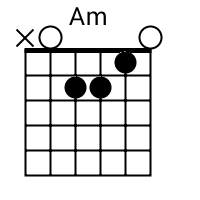
\includegraphics[width=3cm]{../Akordy/am.png}
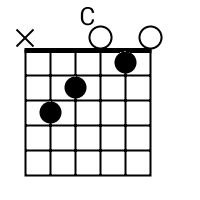
\includegraphics[width=3cm]{../Akordy/c.png}
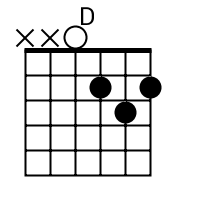
\includegraphics[width=3cm]{../Akordy/d.png}
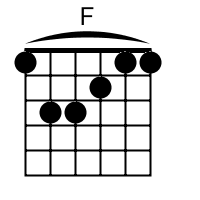
\includegraphics[width=3cm]{../Akordy/f.png}
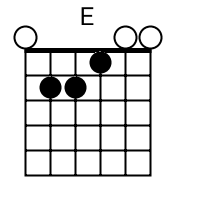
\includegraphics[width=3cm]{../Akordy/e.png}
\end{figure}
\newpage
\addcontentsline{toc}{section}{Houslicky}\begin{song}{title=\centering Housličky \\\normalsize Vlasta Redl  \vspace*{-0.3cm}}  %% sem se napíše jméno songu a autor
\moveright 4cm \vbox{      %Varianta č. 1  ---> Jeden sloupec zarovnaný na střed	

\sloka
^{A}Čí že ste, husličky, ^{D\,\,A\,}čiže,

^{Hmi}kdo vás tu ^{F#mi{\color{white}\_\_}E{\color{white}\_}}zanechal?

^{A}Čí že ste, husličky, ^{D\,\,A\,}čiže,

^{Hmi}kdo vás tu ^{F#mi{\color{white}\_\_}E{\color{white}\_}}zanechal

^{Hmi7}na trávě ^{{\color{white}\_\_}A{\color{white}\_\_}D}poválané,

^{Hmi}na trávě ^{E{\color{white}\_\_}A{\color{white}\_\_}D}poválané,

^{Hmi}u paty ^{F#mi\,\,E{\color{white}\_}}ořecha? ^{Hmi\,\,F#mi\,\,E}


\sloka
A kdože tu trávu tak zválal, aj modré fialy?

A kdože tu trávu tak zválal, aj modré fialy?

že ste, husličky, samé

že ste, husličky, samé na světě zostaly?


\sloka
A který tu muzikant usnul a co sa mu přišlo zdát?

A který tu muzikant usnul a co sa mu přišlo zdát?

Co sa mu enem zdálo, Bože(-)?

Co sa mu enem zdálo, Bože(-), že už vjec nechtěl hrát?


\sloka
Zahrajte, husličky, samy, zahrajte zvesela.

Zahrajte, husličky, samy, zahrajte zvesela.

Až sa tá bude trápit,

až sa tá bude trápit, která ho nechtěla.




}
\setcounter{Slokočet}{0}
\end{song}
\newpage
\addcontentsline{toc}{section}{Huascarán}%%%%%%%%%%%%%%%%%%%%%%%%%%%%%%%%%%%%%%%%%%%%%%%%%%%%%
%			ŠABLONA PÍSNIČEK v. 18.09               %
%%%%%%%%%%%%%%%%%%%%%%%%%%%%%%%%%%%%%%%%%%%%%%%%%%%%%
% Tento soubor slouží jako (naučná) šablona, pomocí 
% které lze vytvářet zdrojové soubory k jednotlivým 
% písním.
%%%%%%%%%%%%%%%%%%%%%%%%%%%%%%%%%%%%%%%%%%%%%%%%%%%%%
%			Jak psát soubory songů?                 %
%%%%%%%%%%%%%%%%%%%%%%%%%%%%%%%%%%%%%%%%%%%%%%%%%%%%%
%	1. Text písně se začíná psát na místě START 
%	   a končí na místě END. Zbylý text ignorujte.
%	2. Jak bude vypadat pdf písně zjistíte po tom, 
%	   co soubor zkompilujete pomocí souboru   
%      ../Generator/generator. 
%	3. Při psaní dodržujte následující TeX pravidla:
%	 a) Nový řádek napíšete pomocí dvou odsazení 
%	    tedy dvou enterů.
%	 b) Nová sloka se píší pomocí \sloka a odsazení.
%		Refrén se píše jako \refren, v případě více 
%		refrénů \refren[č. refrénu].
%	 c) Akordy se píšou tak, že napíšete před slovo,
%	    kde chcete mít akord (bez mezery):
%		^{AKORD1\,AKORD2...}.
%	4. Pokud chcete ušetřit tvůrcům práci, tak 
%	   si přečtěte další poučný soubor o typografii 
%	   ../../Typo_pravidla.txt.
%	5. Akordy stačí psát jen do první sloky, když 
%	   se nezmění -- kytaristé to zvládnou
%	7. Název písně pište na místo [NÁZEV] a autora 
%	   pište na místo [AUTOR] 
%	7. Jak psát věci na české klávesnici:
%	   \ = alt gr + q; [/] = alt gr f/g; 
%      {/} = alt gr + b/n; ^ = alt gr + 3 , cokoliv
%%%%%%%%%%%%%%%%%%%%%%%%%%%%%%%%%%%%%%%%%%%%%%%%%%%%%
%			Jak kompilovat jednotlivé písně?        %
%%%%%%%%%%%%%%%%%%%%%%%%%%%%%%%%%%%%%%%%%%%%%%%%%%%%%
%	1. Více návodu je k tomuto napsáno v souboru 
%      ../Generator/generator. 
%%%%%%%%%%%%%%%%%%%%%%%%%%%%%%%%%%%%%%%%%%%%%%%%%%%%%
%			Jak kompilovat celý zpěvník?			%
%%%%%%%%%%%%%%%%%%%%%%%%%%%%%%%%%%%%%%%%%%%%%%%%%%%%%
%	1. Více návodu je k tomuto napsáno v souboru
%	   ../Cely_zpevnik/zpevnik.tex.
%%%%%%%%%%%%%%%%%%%%%%%%%%%%%%%%%%%%%%%%%%%%%%%%%%%%%
\begin{song}{title=\predtitle \centering Huascarán \\\large  }  %% sem se napíše jméno songu a autor

\vspace*{.5cm}

\begin{centerjustified}
\vetsi
\refren
^{Emi}Od horských ^{D\z}pramenů ^{Emi}Huascarán,

nejtěžší ^{D\z}z~kamenů na ^{\z Emi}prsou mám,

pochází ^{D\z}z~úbočí kde leží ^{Emi\z}cepín tvůj,

slza ^*{\z D}se~r ozskočí, až se vrátíš ^{Emi\z}milý můj.

\sloka
S odvahou zázraků neseš svůj kříž,

k stříbrným oblakům a ještě výš.

Já jsem však zbabělá a tonu v obavách,

čekám tě lásko má, vrať se prosím živ a zdráv.

\ssloka{Recitativ:}
Zpravodajství ČTK: Dne 31. května 1970 vypuklo

v jihoamerické republice Peru katastrofální zemětřesení,

které si vyžádalo tisíce lidských obětí. Mezi nimi i 15 životů

československých horolezců, kteří sem přišli pokořit nejvyšší

horu peruánských And\elipsa.\elipsa.\elipsa.\ Huascarán\elipsa.\elipsa.\elipsa.

\refren

\end{centerjustified}

\setcounter{Slokočet}{0}
\end{song}


\newpage
\addcontentsline{toc}{section}{Hvězdář}%%%%%%%%%%%%%%%%%%%%%%%%%%%%%%%%%%%%%%%%%%%%%%%%%%%%%
%			ŠABLONA PÍSNIČEK v. 18.09               %
%%%%%%%%%%%%%%%%%%%%%%%%%%%%%%%%%%%%%%%%%%%%%%%%%%%%%
% Tento soubor slouží jako (naučná) šablona, pomocí 
% které lze vytvářet zdrojové soubory k jednotlivým 
% písním.
%%%%%%%%%%%%%%%%%%%%%%%%%%%%%%%%%%%%%%%%%%%%%%%%%%%%%
%			Jak psát soubory songů?                 %
%%%%%%%%%%%%%%%%%%%%%%%%%%%%%%%%%%%%%%%%%%%%%%%%%%%%%
%	1. Text písně se začíná psát na místě START 
%	   a končí na místě END. Zbylý text ignorujte.
%	2. Jak bude vypadat pdf písně zjistíte po tom, 
%	   co soubor zkompilujete pomocí souboru   
%      ../Generator/generator. 
%	3. Při psaní dodržujte následující TeX pravidla:
%	 a) Nový řádek napíšete pomocí dvou odsazení 
%	    tedy dvou enterů.
%	 b) Nová sloka se píší pomocí \sloka a odsazení.
%		Refrén se píše jako \refren, v případě více 
%		refrénů \refren[č. refrénu].
%	 c) Akordy se píšou tak, že napíšete před slovo,
%	    kde chcete mít akord (bez mezery):
%		^{AKORD1\,AKORD2...}.
%	4. Pokud chcete ušetřit tvůrcům práci, tak 
%	   si přečtěte další poučný soubor o typografii 
%	   ../../Typo_pravidla.txt.
%	5. Akordy stačí psát jen do první sloky, když 
%	   se nezmění -- kytaristé to zvládnou
%	7. Název písně pište na místo [NÁZEV] a autora 
%	   pište na místo [AUTOR] 
%	7. Jak psát věci na české klávesnici:
%	   \ = alt gr + q; [/] = alt gr f/g; 
%      {/} = alt gr + b/n; ^ = alt gr + 3 , cokoliv
%%%%%%%%%%%%%%%%%%%%%%%%%%%%%%%%%%%%%%%%%%%%%%%%%%%%%
%			Jak kompilovat jednotlivé písně?        %
%%%%%%%%%%%%%%%%%%%%%%%%%%%%%%%%%%%%%%%%%%%%%%%%%%%%%
%	1. Více návodu je k tomuto napsáno v souboru 
%      ../Generator/generator. 
%%%%%%%%%%%%%%%%%%%%%%%%%%%%%%%%%%%%%%%%%%%%%%%%%%%%%
%			Jak kompilovat celý zpěvník?			%
%%%%%%%%%%%%%%%%%%%%%%%%%%%%%%%%%%%%%%%%%%%%%%%%%%%%%
%	1. Více návodu je k tomuto napsáno v souboru
%	   ../Cely_zpevnik/zpevnik.tex.
%%%%%%%%%%%%%%%%%%%%%%%%%%%%%%%%%%%%%%%%%%%%%%%%%%%%%
\begin{song}{title=\predtitle \centering Hvězdář \\\large UDG }  %% sem se napíše jméno songu a autor

\vspace*{.5cm}

\begin{centerjustified}
\vetsi
\sloka
Ztrácíš se ^{D\z}před očima, rosteš jen ^{A}ve vlastním stínu.

Každá ^{Emi\z}další vina, odkrývá ^{Cmaj7}mojí vinu.

Ztrácíš se před očima, rosteš jen ve vlastním stínu.

Každá další vina odkrývá mojí vinu.

\sloka
/: Ve vínu dávno nic nehledám, (dávno nic) nehledám. :/

\refren
Jak luna mizíš s nocí v bělostných šatech pro nemocné,

prosit je zvláštní pocit, jen ať je den noc ne.

Jak luna mizíš s nocí v bělostných šatech pro nemocné,

prosit je zvláštní pocit, jen ať je den noc ne.

\sloka
/: Od proseb dávno nic nečekám (dávno nic) nečekám. :/

\ssloka{Mezihra:}
\textbf{D A Emi Cmaj7 D A Emi Cmaj7}

\sloka
Na chodbách v bludných kruzích zářivka vyhasíná,

já ti do infuzí chci přilít trochu vína.

Na nebi jiných sluncí, jak se tam asi cítíš,

s nebeskou interpunkcí, jiným tulákům svítíš.

\sloka
/: Ve vínu dávno nic nehledám (dávno nic) nehledám. :/

\refren

\sloka
Obzor neklesne níž, je ráno a ty spíš.

Od vlků odraná hvězdáře Giordána\dots

Obzor neklesne níž, je ráno a ty spíš.

Od vlků odraná hvězdáře Giordána\dots

Obzor neklesne níž, je ráno a ty spíš.

Od vlků odraná hvězdáře Giordána\elipsa.\elipsa.\elipsa.~opouštíš.

\end{centerjustified}

\setcounter{Slokočet}{0}
\end{song}


\newpage
\addcontentsline{toc}{section}{Chci ti říct}\begin{song}{title=\predtitle\centering Chci ti říct \\\large Mig 21  \vspace*{-0.3cm}}  %% sem se napíše jméno songu a autor
\begin{centerjustified}


\predehra
4$\times $\textbf{Gmi C2}

\sloka
	^{Gmi}Chladná ^{C2}rána jsou ^{Gmi}tomu, kdo ^{C2}strádá,

	^{Gmi\,\,}láskou ^{C2\z }bolestnou ^{Gmi\z C2}neopětovanou.

	Pokud ^{Gmi}víš, jak ^{C2}rád tě mám, ^{Gmi}a ty mě máš ^{C2}ráda.

	^{Gmi}Chuť a ^{C2}vůni tvou ^{Gmi}nejde ^{C2\z }zapomenout.

\sloka
	Chystá ^{Dmi}se prej konec ^{C2}světa, ^{Gmi}tramtadá

	a ^{Dmi}mě jen jedna ^{C2}věta ^{\z B2}napadá. (\dots\,tak pojď s tim ven!)

\refren
	^{F}Chci ti říct, že mám tě ^{C2}rád, že ^{Gmi}miluju tě jako blázen,

	^{F}chci si nechat ^{C2\z }tetovat jen ^{Gmi}jméno tvé, chci vypít bazén

	^{F}vody, kterou ^{C2\z }plavala jsi, ^{Gmi\z }zasadit si tvoje vlasy,

	^{F\z }rozfoukat je ^{C2}do ulic ^{Gmi}chci ti říct, že rád tě mám ^{B7}víc.

\sloka
	Dýcháš na mou tvář, já na tvou dýchám.

	Chvěješ se myšlenkou, že se rozední.

	Děláš, jako že nespěcháš, já že nepospíchám.

	Nechce se z objetí, když je poslední.

\sloka  = 2.

\refren


\sloka
	/: ^{B7}Mít tak promyšlenej plán, předem fakt moc se omlouvám, 

	ale ode dneška od půl jedný musíme bejt zodpovědný. :/

	^{B7}Mít tak promyšlenej plán, ale nemám ho, nemám ho, nemám\elipsa.\elipsa.\elipsa.\,a tak:

\refren


\end{centerjustified}
\setcounter{Slokočet}{0}
\end{song}
\newpage
\addcontentsline{toc}{section}{Chvíle}%%%%%%%%%%%%%%%%%%%%%%%%%%%%%%%%%%%%%%%%%%%%%%%%%%%%%
%			ŠABLONA PÍSNIČEK v. 18.09               %
%%%%%%%%%%%%%%%%%%%%%%%%%%%%%%%%%%%%%%%%%%%%%%%%%%%%%
% Tento soubor slouží jako (naučná) šablona, pomocí 
% které lze vytvářet zdrojové soubory k jednotlivým 
% písním.
%%%%%%%%%%%%%%%%%%%%%%%%%%%%%%%%%%%%%%%%%%%%%%%%%%%%%
%			Jak psát soubory songů?                 %
%%%%%%%%%%%%%%%%%%%%%%%%%%%%%%%%%%%%%%%%%%%%%%%%%%%%%
%	1. Text písně se začíná psát na místě START 
%	   a končí na místě END. Zbylý text ignorujte.
%	2. Jak bude vypadat pdf písně zjistíte po tom, 
%	   co soubor zkompilujete pomocí souboru   
%      ../Generator/generator. 
%	3. Při psaní dodržujte následující TeX pravidla:
%	 a) Nový řádek napíšete pomocí dvou odsazení 
%	    tedy dvou enterů.
%	 b) Nová sloka se píší pomocí \sloka a odsazení.
%		Refrén se píše jako \refren, v případě více 
%		refrénů \refren[č. refrénu].
%	 c) Akordy se píšou tak, že napíšete před slovo,
%	    kde chcete mít akord (bez mezery):
%		^{AKORD1\,AKORD2...}.
%	4. Pokud chcete ušetřit tvůrcům práci, tak 
%	   si přečtěte další poučný soubor o typografii 
%	   ../../Typo_pravidla.txt.
%	5. Akordy stačí psát jen do první sloky, když 
%	   se nezmění -- kytaristé to zvládnou
%	7. Název písně pište na místo [NÁZEV] a autora 
%	   pište na místo [AUTOR] 
%	7. Jak psát věci na české klávesnici:
%	   \ = alt gr + q; [/] = alt gr f/g; 
%      {/} = alt gr + b/n; ^ = alt gr + 3 , cokoliv
%%%%%%%%%%%%%%%%%%%%%%%%%%%%%%%%%%%%%%%%%%%%%%%%%%%%%
%			Jak kompilovat jednotlivé písně?        %
%%%%%%%%%%%%%%%%%%%%%%%%%%%%%%%%%%%%%%%%%%%%%%%%%%%%%
%	1. Více návodu je k tomuto napsáno v souboru 
%      ../Generator/generator. 
%%%%%%%%%%%%%%%%%%%%%%%%%%%%%%%%%%%%%%%%%%%%%%%%%%%%%
%			Jak kompilovat celý zpěvník?			%
%%%%%%%%%%%%%%%%%%%%%%%%%%%%%%%%%%%%%%%%%%%%%%%%%%%%%
%	1. Více návodu je k tomuto napsáno v souboru
%	   ../Cely_zpevnik/zpevnik.tex.
%%%%%%%%%%%%%%%%%%%%%%%%%%%%%%%%%%%%%%%%%%%%%%%%%%%%%
\begin{song}{title=\predtitle \centering Chvíle \\\large Hop trop }  %% sem se napíše jméno songu a autor

\vspace*{.5cm}

\begin{centerjustified}
\vetsi
\sloka
^{Emi}Mám rád ty chvíle, kdy noc už pomalu ^{Hmi}končí,

^{\z Ami}chvíle, co patřej' jen ^{\z Hmi}těm, co ^{\z Emi}neusínaj',

toulavejm bláznům, když právě s jarem se ^{Hmi}loučí

a ^{Ami\z}za~dobrý slovo ti ^{Hmi}srdce svý na dlani ^{Emi}daj'.

\sloka
Mám rád ty chvíle, kdy holkám ve vočích svítí

slunce, když do korun stromů začlo se drát,

stejně jak v kapičkách rosy na pavoučích sítích,

to najednou chce se mi brečet a zároveň smát.

\refren
Ty rána s ^{A}vůní borový ^{\z Emi}smůly

měly by ^{A\z}zůstat navždycky v ^{\z Emi}nás,

ty rána s ^{C\z}vůní sekaný ^{Hmi}trávy

a ohně, co ^{C}právě ^{Hmi}pomalu ^{\z Emi}zhas'.

\sloka
Mám rád ty chvíle, kdy kluci v duchu si říkaj',

jak je to nádherný, léto před sebou mít,

spolu si přejou, ať moc rychle dny neutíkaj'

a trápení jsou někde v dálce, a kolem je klid.

\sloka = 1.

\refren

\end{centerjustified}

\setcounter{Slokočet}{0}
\end{song}


\newpage
\addcontentsline{toc}{section}{Jacek}%%%%%%%%%%%%%%%%%%%%%%%%%%%%%%%%%%%%%%%%%%%%%%%%%%%%%
%			ŠABLONA PÍSNIČEK v. 18.09               %
%%%%%%%%%%%%%%%%%%%%%%%%%%%%%%%%%%%%%%%%%%%%%%%%%%%%%
% Tento soubor slouží jako (naučná) šablona, pomocí 
% které lze vytvářet zdrojové soubory k jednotlivým 
% písním.
%%%%%%%%%%%%%%%%%%%%%%%%%%%%%%%%%%%%%%%%%%%%%%%%%%%%%
%			Jak psát soubory songů?                 %
%%%%%%%%%%%%%%%%%%%%%%%%%%%%%%%%%%%%%%%%%%%%%%%%%%%%%
%	1. Text písně se začíná psát na místě START 
%	   a končí na místě END. Zbylý text ignorujte.
%	2. Jak bude vypadat pdf písně zjistíte po tom, 
%	   co soubor zkompilujete pomocí souboru   
%      ../Generator/generator. 
%	3. Při psaní dodržujte následující TeX pravidla:
%	 a) Nový řádek napíšete pomocí dvou odsazení 
%	    tedy dvou enterů.
%	 b) Nová sloka se píší pomocí \sloka a odsazení.
%		Refrén se píše jako \refren, v případě více 
%		refrénů \refren[č. refrénu].
%	 c) Akordy se píšou tak, že napíšete před slovo,
%	    kde chcete mít akord (bez mezery):
%		^{AKORD1\,AKORD2...}.
%	4. Pokud chcete ušetřit tvůrcům práci, tak 
%	   si přečtěte další poučný soubor o typografii 
%	   ../../Typo_pravidla.txt.
%	5. Akordy stačí psát jen do první sloky, když 
%	   se nezmění -- kytaristé to zvládnou
%	7. Název písně pište na místo [NÁZEV] a autora 
%	   pište na místo [AUTOR] 
%	7. Jak psát věci na české klávesnici:
%	   \ = alt gr + q; [/] = alt gr f/g; 
%      {/} = alt gr + b/n; ^ = alt gr + 3 , cokoliv
%%%%%%%%%%%%%%%%%%%%%%%%%%%%%%%%%%%%%%%%%%%%%%%%%%%%%
%			Jak kompilovat jednotlivé písně?        %
%%%%%%%%%%%%%%%%%%%%%%%%%%%%%%%%%%%%%%%%%%%%%%%%%%%%%
%	1. Více návodu je k tomuto napsáno v souboru 
%      ../Generator/generator. 
%%%%%%%%%%%%%%%%%%%%%%%%%%%%%%%%%%%%%%%%%%%%%%%%%%%%%
%			Jak kompilovat celý zpěvník?			%
%%%%%%%%%%%%%%%%%%%%%%%%%%%%%%%%%%%%%%%%%%%%%%%%%%%%%
%	1. Více návodu je k tomuto napsáno v souboru
%	   ../Cely_zpevnik/zpevnik.tex.
%%%%%%%%%%%%%%%%%%%%%%%%%%%%%%%%%%%%%%%%%%%%%%%%%%%%%
\vspace{-.5cm}
\begin{song}{title=\predtitle \centering Jacek \\\large Jaromír Nohavica }  %% sem se napíše jméno songu a autor

\vspace*{-.5cm}

\begin{centerjustified}
\vetsi
\sloka
^{G}Na druhém břehu řeky ^{D\z}Olše žije Jacek,

^{C}mám k němu stejně blízko ^{G}jak on ke mně,

^{G}máváme na sebe z ^{D}říční navigace,

^{C\z}dva spojenci a dvě ^*{\z G}spřá telené země,

jak malí kluci hážem z ^{D}břehů žabky,

^{C\z}kdo vyhraje, má z ^*{\z G}protější ho srandu,

hlavama kroutí česko-polské babky,

^*{C}dě láme prostě vlastní ^*{\z G}pro pagandu.

\sloka
Na mostě přátelství se tvoří dlouhé fronty

všelikých věcí za všelikou cenu,

já mám však na to velmi úzké horizonty

a Jacek velmi nenáročnou ženu,

týden co týden z břehů navigace

na sebe řveme:\uv{Chlapče, hlavu vzhůru!},

jak je to krásné, moci vykašlat se

na celní předpisy a na cenzuru, na na\elipsa.\elipsa.\elipsa.

\sloka
Z Piastovské věže na nás mává kníže Měšek

a směje se, až třepe se mu brada,

ve zprávách večer běží horký dnešek,

aspoň se máme s Jackem o co hádat,

on tvrdí svoje, já zas tvrdím svoje

a domluvit se někdy bývá marno,

tak spolu vedem pohraniční boje

a v praxi demonstrujem Solidarnosc, na na\elipsa.\elipsa.\elipsa.

\sloka
Na druhém břehu řeky Olše žije Jacek,

mám k němu stejně blízko jak on ke mně,

máváme na sebe z říční navigace,

dva spojenci a dvě spřátelené země

/: a voda plyne, plyne, plyne dlouhé věky,

řeka se kroutí jako modrá šňůrka

a my dva hážem kachnám vprostřed řeky

krajíčky chleba o dvou stejných kůrkách. :/

Na na na\elipsa.\elipsa.\elipsa.



\end{centerjustified}
\setcounter{Slokočet}{0}
\end{song}


\newpage
\addcontentsline{toc}{section}{Jahody Mražený}%%%%%%%%%%%%%%%%%%%%%%%%%%%%%%%%%%%%%%%%%%%%%%%%%%%%%
%			ŠABLONA PÍSNIČEK v. 18.09               %
%%%%%%%%%%%%%%%%%%%%%%%%%%%%%%%%%%%%%%%%%%%%%%%%%%%%%
% Tento soubor slouží jako (naučná) šablona, pomocí 
% které lze vytvářet zdrojové soubory k jednotlivým 
% písním.
%%%%%%%%%%%%%%%%%%%%%%%%%%%%%%%%%%%%%%%%%%%%%%%%%%%%%
%			Jak psát soubory songů?                 %
%%%%%%%%%%%%%%%%%%%%%%%%%%%%%%%%%%%%%%%%%%%%%%%%%%%%%
%	1. Text písně se začíná psát na místě START 
%	   a končí na místě END. Zbylý text ignorujte.
%	2. Jak bude vypadat pdf písně zjistíte po tom, 
%	   co soubor zkompilujete pomocí souboru   
%      ../Generator/generator. 
%	3. Při psaní dodržujte následující TeX pravidla:
%	 a) Nový řádek napíšete pomocí dvou odsazení 
%	    tedy dvou enterů.
%	 b) Nová sloka se píší pomocí \sloka a odsazení.
%		Refrén se píše jako \refren, v případě více 
%		refrénů \refren[č. refrénu].
%	 c) Akordy se píšou tak, že napíšete před slovo,
%	    kde chcete mít akord (bez mezery):
%		^{AKORD1\,AKORD2...}.
%	4. Pokud chcete ušetřit tvůrcům práci, tak 
%	   si přečtěte další poučný soubor o typografii 
%	   ../../Typo_pravidla.txt.
%	5. Akordy stačí psát jen do první sloky, když 
%	   se nezmění -- kytaristé to zvládnou
%	7. Název písně pište na místo [NÁZEV] a autora 
%	   pište na místo [AUTOR] 
%	7. Jak psát věci na české klávesnici:
%	   \ = alt gr + q; [/] = alt gr f/g; 
%      {/} = alt gr + b/n; ^ = alt gr + 3 , cokoliv
%%%%%%%%%%%%%%%%%%%%%%%%%%%%%%%%%%%%%%%%%%%%%%%%%%%%%
%			Jak kompilovat jednotlivé písně?        %
%%%%%%%%%%%%%%%%%%%%%%%%%%%%%%%%%%%%%%%%%%%%%%%%%%%%%
%	1. Více návodu je k tomuto napsáno v souboru 
%      ../Generator/generator. 
%%%%%%%%%%%%%%%%%%%%%%%%%%%%%%%%%%%%%%%%%%%%%%%%%%%%%
%			Jak kompilovat celý zpěvník?			%
%%%%%%%%%%%%%%%%%%%%%%%%%%%%%%%%%%%%%%%%%%%%%%%%%%%%%
%	1. Více návodu je k tomuto napsáno v souboru
%	   ../Cely_zpevnik/zpevnik.tex.
%%%%%%%%%%%%%%%%%%%%%%%%%%%%%%%%%%%%%%%%%%%%%%%%%%%%%
\begin{song}{title=\predtitle \centering Jahody mražený \\\large Jiří Schelinger }  %% sem se napíše jméno songu a autor

\vspace*{.5cm}

\begin{centerjustified}
\vetsi
\sloka
^{A\z }Poslala mě moje dívka ^{D\z }pro jahody ^*{\z A}červen ý,

^{D}bez nich se prý nemám ^{G\z}vracet, ^{A\z}tak tu stojím ztrápený.

Když se dívám co je sněhu, ^{D\z}fouká vítr, pálí ^{A\z}mráz,

^{D\z}možná že si děvče ^{G\z}myslí, ^{A}že se mě tak zbaví ^{E\z}snáz.

\refren
/: ^{G\z}Zapomněla ^*{\z D}váže ní, ^{A}na jahody ^*{E}mražen ý,

^{G}na jahody ^*{\z D}mražený , ^{A\z}v~igelitu ^*{\z E}balený . :/

\sloka
Pohádku to připomíná o dvanácti měsíčkách,

nechtěla mi říci sbohem, teď by chtěla, abych plách.

Mohl bych se klidně vrátit, vím však, že mě nečeká,

měla mi to říci rovnou, že jiného ráda má.


\refren

\refren

\end{centerjustified}
\setcounter{Slokočet}{0}
\end{song}
\newpage
\addcontentsline{toc}{section}{Jdem zpátky do lesů}%%%%%%%%%%%%%%%%%%%%%%%%%%%%%%%%%%%%%%%%%%%%%%%%%%%%%
%			ŠABLONA PÍSNIČEK v. 18.09               %
%%%%%%%%%%%%%%%%%%%%%%%%%%%%%%%%%%%%%%%%%%%%%%%%%%%%%
% Tento soubor slouží jako (naučná) šablona, pomocí 
% které lze vytvářet zdrojové soubory k jednotlivým 
% písním.
%%%%%%%%%%%%%%%%%%%%%%%%%%%%%%%%%%%%%%%%%%%%%%%%%%%%%
%			Jak psát soubory songů?                 %
%%%%%%%%%%%%%%%%%%%%%%%%%%%%%%%%%%%%%%%%%%%%%%%%%%%%%
%	1. Text písně se začíná psát na místě START 
%	   a končí na místě END. Zbylý text ignorujte.
%	2. Jak bude vypadat pdf písně zjistíte po tom, 
%	   co soubor zkompilujete pomocí souboru   
%      ../Generator/generator. 
%	3. Při psaní dodržujte následující TeX pravidla:
%	 a) Nový řádek napíšete pomocí dvou odsazení 
%	    tedy dvou enterů.
%	 b) Nová sloka se píší pomocí \sloka a odsazení.
%		Refrén se píše jako \refren, v případě více 
%		refrénů \refren[č. refrénu].
%	 c) Akordy se píšou tak, že napíšete před slovo,
%	    kde chcete mít akord (bez mezery):
%		^{AKORD1\,AKORD2...}.
%	4. Pokud chcete ušetřit tvůrcům práci, tak 
%	   si přečtěte další poučný soubor o typografii 
%	   ../../Typo_pravidla.txt.
%	5. Akordy stačí psát jen do první sloky, když 
%	   se nezmění -- kytaristé to zvládnou
%	7. Název písně pište na místo [NÁZEV] a autora 
%	   pište na místo [AUTOR] 
%	7. Jak psát věci na české klávesnici:
%	   \ = alt gr + q; [/] = alt gr f/g; 
%      {/} = alt gr + b/n; ^ = alt gr + 3 , cokoliv
%%%%%%%%%%%%%%%%%%%%%%%%%%%%%%%%%%%%%%%%%%%%%%%%%%%%%
%			Jak kompilovat jednotlivé písně?        %
%%%%%%%%%%%%%%%%%%%%%%%%%%%%%%%%%%%%%%%%%%%%%%%%%%%%%
%	1. Více návodu je k tomuto napsáno v souboru 
%      ../Generator/generator. 
%%%%%%%%%%%%%%%%%%%%%%%%%%%%%%%%%%%%%%%%%%%%%%%%%%%%%
%			Jak kompilovat celý zpěvník?			%
%%%%%%%%%%%%%%%%%%%%%%%%%%%%%%%%%%%%%%%%%%%%%%%%%%%%%
%	1. Více návodu je k tomuto napsáno v souboru
%	   ../Cely_zpevnik/zpevnik.tex.
%%%%%%%%%%%%%%%%%%%%%%%%%%%%%%%%%%%%%%%%%%%%%%%%%%%%%
\begin{song}{title=\predtitle \centering Jdem zpátky do lesů \\\large Žalman }  %% sem se napíše jméno songu a autor

\vspace*{.5cm}

\begin{centerjustified}
\vetsi
\sloka
^{Ami7}Sedím na kolejích, ^{D}které nikam ^{\z G C G}nevedou,~~~~~~

koukám na kopretinu, jak miluje se s lebedou,

^{Ami7}mraky vzaly slunce ^*{D}za se pod svou ^{\z G Emi}ochranu,~~~~~~~

^{Ami7}jen~ty nejdeš, holka zlatá, ^{D}kdypak já tě ^{\z G D}dostanu?~~~

\refren
Z ^{G}ráje, my vyhnaní z ^{Emi}ráje,

kde není už ^{Ami7}místa, ^*{\z C7}prej\: něco se ^{\z G\phantom{G} D}chystá,~~

z ^{G}ráje nablýskaných ^{Emi}plesů,

jdem zpátky do ^*{Ami C7}lesů~za~něj aký ^{G}čas.

\sloka
Vlak nám včera ujel ze stanice do nebe,

málo jsi se snažil, málo šel jsi do sebe,

šel jsi vlastní cestou, a to se zrovna nenosí,

i pes, kterej chce přízeň, napřed svýho pána poprosí.

\refren

\sloka
Už tě vidím z dálky, jak máváš na mě korunou,

a jestli nám to bude stačit, zatleskáme na druhou,

zabalíme všechny, co si dávaj' rande za branou,

v ráji není místa, možná v pekle se nás zastanou.

\refren

\end{centerjustified}
\setcounter{Slokočet}{0}
\end{song}
\newpage
\addcontentsline{toc}{section}{Ještě jedno kafe}\begin{song}{title=\predtitle\centering Ještě jedno kafe  \\\large Druhá Tráva a Robert Křesťan  \vspace*{-0.3cm}}  %% sem se napíše jméno songu a autor
\begin{centerjustified}
\nejnejvetsi

\sloka 
	Máš ^*{Emi}sladk ej dech a oči, kterým ^*{D}pa tří svatozář

	a ^*{C}vl asy máš jak hedvábí, když je ^*{H7}vho díš na polštář,

	ale ^{Emi}já se o tvou lásku ani ^*{D}vd ěčnost neprosím,

	ty ^*{C}dě kuješ jen hvězdám a jseš ^*{H7}věr ná jenom jim.

\refren
	^*{C}Je ště jedno kafe bych si ^{H7}dal,

	^*{C}je ště jedno kafe, ^{{\color{white}\_\_\_}H7}krucinál, než pojedu ^{Emi}dál.

\sloka
	Tvůj táta, to je vandrák a od přírody zběh
	
	a místo písmen učí tě jen dorovnávat dech
	
	a taky házet nožem a držet pospolu
   
	a brada se mu třese, když se nosí ke stolu.

\refren


\sloka
	Tvá sestra hádá z ruky a tvá máti jakbysmet
	
	a ty sama umíš všechno, co je mimo tenhle svět,
	
	a tvá rozkoš nezná hranic, děvče s hlasem skřivana.
	
	Jen tvý srdce je jak moře -- samý tajemství a tma.

\refren


\end{centerjustified}
\setcounter{Slokočet}{0}
\end{song}
\newpage
\addcontentsline{toc}{section}{Jožin z bažin}%%%%%%%%%%%%%%%%%%%%%%%%%%%%%%%%%%%%%%%%%%%%%%%%%%%%%
%			ŠABLONA PÍSNIČEK v. 18.09               %
%%%%%%%%%%%%%%%%%%%%%%%%%%%%%%%%%%%%%%%%%%%%%%%%%%%%%
% Tento soubor slouží jako (naučná) šablona, pomocí 
% které lze vytvářet zdrojové soubory k jednotlivým 
% písním.
%%%%%%%%%%%%%%%%%%%%%%%%%%%%%%%%%%%%%%%%%%%%%%%%%%%%%
%			Jak psát soubory songů?                 %
%%%%%%%%%%%%%%%%%%%%%%%%%%%%%%%%%%%%%%%%%%%%%%%%%%%%%
%	1. Text písně se začíná psát na místě START 
%	   a končí na místě END. Zbylý text ignorujte.
%	2. Jak bude vypadat pdf písně zjistíte po tom, 
%	   co soubor zkompilujete pomocí souboru   
%      ../Generator/generator. 
%	3. Při psaní dodržujte následující TeX pravidla:
%	 a) Nový řádek napíšete pomocí dvou odsazení 
%	    tedy dvou enterů.
%	 b) Nová sloka se píší pomocí \sloka a odsazení.
%		Refrén se píše jako \refren, v případě více 
%		refrénů \refren[č. refrénu].
%	 c) Akordy se píšou tak, že napíšete před slovo,
%	    kde chcete mít akord (bez mezery):
%		^{AKORD1\,AKORD2...}.
%	4. Pokud chcete ušetřit tvůrcům práci, tak 
%	   si přečtěte další poučný soubor o typografii 
%	   ../../Typo_pravidla.txt.
%	5. Akordy stačí psát jen do první sloky, když 
%	   se nezmění -- kytaristé to zvládnou
%	7. Název písně pište na místo [NÁZEV] a autora 
%	   pište na místo [AUTOR] 
%	7. Jak psát věci na české klávesnici:
%	   \ = alt gr + q; [/] = alt gr f/g; 
%      {/} = alt gr + b/n; ^ = alt gr + 3 , cokoliv
%%%%%%%%%%%%%%%%%%%%%%%%%%%%%%%%%%%%%%%%%%%%%%%%%%%%%
%			Jak kompilovat jednotlivé písně?        %
%%%%%%%%%%%%%%%%%%%%%%%%%%%%%%%%%%%%%%%%%%%%%%%%%%%%%
%	1. Více návodu je k tomuto napsáno v souboru 
%      ../Generator/generator. 
%%%%%%%%%%%%%%%%%%%%%%%%%%%%%%%%%%%%%%%%%%%%%%%%%%%%%
%			Jak kompilovat celý zpěvník?			%
%%%%%%%%%%%%%%%%%%%%%%%%%%%%%%%%%%%%%%%%%%%%%%%%%%%%%
%	1. Více návodu je k tomuto napsáno v souboru
%	   ../Cely_zpevnik/zpevnik.tex.
%%%%%%%%%%%%%%%%%%%%%%%%%%%%%%%%%%%%%%%%%%%%%%%%%%%%%
\begin{song}{title=\predtitle \centering Jožin z bažin \\\large Ivan Mládek }  %% sem se napíše jméno songu a autor

\vspace*{.5cm}
\moveright .5cm \vbox{
\begin{centerjustified}
\vetsi
\sloka
^{Emi \z}Jedu takhle tábořit Škodou 100 na ^{Emi\z }Oravu,

spěchám proto, riskuji, ^{H7\z}projíždím přes ^{Emi \z}Moravu.

^{D7}Řádí tam to ^{G\z}strašidlo, ^{D7\z}vystupuje z ^{G H7\z}bažin,

^{Emi\z}žere hlavně Pražáky, ^{H7\z}jmenuje se ^{Emi D7}Jožin.~~

\refren
^{G\z}Jožin z bažin močálem se ^{D7\z}plíží,

Jožin z bažin k vesnici se ^{G\z}blíží,

Jožin z bažin už si zuby ^{D7\z}brousí,

Jožin z bažin kouše, saje, ^{G\z}rdousí.

^{C}Na Jožina z ^{G\z}bažin, ^{D\z}koho by to ^{\z G}napadlo,

^{C\z}platí jen a ^{G\z}pouze ^{D\z}práškovací ^{G H7 Emi}letadlo.~~~~~~~~~~~~~~~~~

\sloka
Projížděl jsem dědinou cestou na Vizovice,

přivítal mě předseda, řek' mi u slivovice:

\uv{Živého či mrtvého Jožina kdo přivede,

tomu já dám za ženu dceru a půl JZD!}

\refren

\sloka
Říkám:\uv{Dej mi, předsedo, letadlo a prášek,

Jožina ti přivedu, nevidím v tom háček.}

Předseda mi vyhověl, ráno jsem se vznesl,

na Jožina z letadla prášek pěkně klesl.

\refren
Jožin z bažin už je celý bílý,

Jožin z bažin z močálu ven pílí,

Jožin z bažin dostal se na kámen,

Jožin z bažin -- tady je s ním amen!

Jožina jsem dohnal, už ho držím, johoho,

dobré každé lóve, prodám já ho do ZOO.

\end{centerjustified}
}
\setcounter{Slokočet}{0}
\end{song}
\newpage
\addcontentsline{toc}{section}{Kluziště}\begin{song}{title=\centering Kluziště \\\normalsize Karel Plíhal \vspace*{-0.3cm}}  %% sem se napíše jméno songu a autor
\moveright 4cm \vbox{      %Varianta č. 1  ---> Jeden sloupec zarovnaný na střed	

\sloka 
	^{C{\color{white}aaaa}}Strejček ^{Emi7/H}kovář ^{Ami7}chytil ^{C/G}kleště, 

	^{Fmaj7}uštíp' z ^{C}noční ^{\,\,\,Fmaj7\,\,G}oblohy
	
	jednu malou kapku deště, ta mu spadla pod nohy.
	
	Nejdřív ale chytil slinu, tak šáh' kamsi pro pivo,
	
	pak přitáhl kovadlinu a obrovský kladivo.

\refren
	Zatím ^{C}tři bílé ^{Emi7/H}vrány ^{Ami7}pěkně za ^{C/G}sebou
	
	kolem ^{Fmaj7}jdou, někam ^{C}jdou, do ^{D7}rytmu se ^{G}kývají,

	tyhle ^{C}tři bílé ^{Emi7/H}vrány ^{Ami7}pěkně za ^{C/G}sebou
	
	kolem ^{Fmaj7}jdou, někam ^{C}jdou, ^{Fmaj7}nedojdou, ^{C}nedojdou.


\sloka	
	Vydal z hrdla mocný pokřik ztichlým letním večerem,
	
	pak tu kapku všude rozstřík' jedním mocným úderem.
	
	Celej svět byl náhle v kapce a vysoko nad námi.
	
	Na obrovské mucholapce visí nebe s hvězdami.

\refren

\sloka
	Zpod víček mi vytrysk' pramen na zmačkané polštáře,
	
	kdosi mě vzal kolem ramen a políbil na tváře,
	
	kdesi v dálce rozmazaně strejda kovář odchází,
	
	do kalhot si čistí dlaně umazané od sazí. 


}
\setcounter{Slokočet}{0}

\begin{center}
	\vspace*{1.0in}
	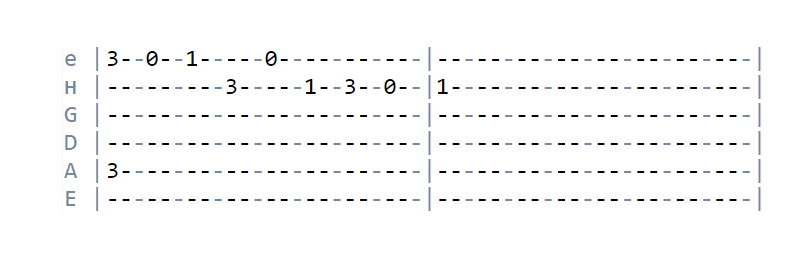
\includegraphics[scale=0.5]{../taby/kluziste.PNG}

\end{center}

	
\end{song}


\newpage	
\addcontentsline{toc}{section}{Kometa}\begin{song}{title=\centering Kometa \\\normalsize Jaromír Nohavica \vspace*{-0.3cm}}  %% sem se napíše jméno songu a autor
\moveright 1cm \vbox{      %Varianta č. 1  ---> Jeden sloupec zarovnaný na střed	
\begin{minipage}[t]{0.48\textwidth}\setlength{\parindent}{0.45cm}  %Varianta č. 2 --> Dva sloupce

\sloka 
	^{Ami{\color{white}\_}}Spatřil jsem kometu, oblohou letěla,
	
	chtěl jsem jí zazpívat, ona mi zmizela.
	
	^{Dmi{\color{white}\_}}Zmizela jako laň ^{G7}u lesa v remízku,
	
	^{C}v očích mi zbylo jen ^{E7}pár žlutých penízků.

\sloka
	Penízky ukryl jsem do hlíny pod dubem,
	
	až příště přiletí, my už tu nebudem.
	
	My už tu nebudem, ach, pýcho marnivá,
	
	spatřil jsem kometu, chtěl jsem jí 
	
	zazpívat.
	
\refren
	^{Ami}O vodě, o trávě, ^{Dmi}o lese,
	
	^{G7}o smrti, se kterou smířit ^{C\,\,\,\,\,\,}nejde se,
	
	^{Ami}o lásce, o zradě, ^{Dmi}o světě
	
	^{E}a o všech lidech, co kdy ^{E7}žili na téhle 
	
	 ^{Ami\,\,\,\,\,\,}planetě.
	
\sloka	
	Na hvězdném nádraží cinkají vagóny,
	
	pan Kepler rozepsal nebeské zákony,
	
	hledal, až nalezl v hvězdářských triedrech
	
	tajemství, která teď neseme na bedrech.

\sloka
	Velká a odvěká tajemství přírody,
	
	že jenom z člověka člověk se narodí,
	
	že kořen s větvemi ve strom se spojuje
	
	a krev našich nadějí vesmírem putuje.

\refren
Na na na\elipsa\dots

\sloka
	Spatřil jsem kometu, byla jak reliéf
	
	zpod rukou umělce, který už nežije,
	
	šplhal jsem do nebe, chtěl jsem ji osahat,
	
	marnost mne vysvlékla celého donaha.
	
\end{minipage}\begin{minipage}[t]{0.5\textwidth}\setlength{\parindent}{0.45cm}\vspace*{0.55cm}  % V případě varianty č.2 jde odsud text do pravé části

\sloka
	Jak socha Davida z bílého mramoru
	
	stál jsem a hleděl jsem, hleděl jsem nahoru.
	
	Až příště přiletí, ach, pýcho marnivá,
	
	my už tu nebudem, ale jiný jí zazpívá.


\refren
	O vodě, o trávě, o lese,
	
	o smrti, se kterou smířit nejde se,
	
	o lásce, o zradě, o světě,
	
	bude to písnička o nás a kometě\elipsa\dots

\end{minipage}
}
\setcounter{Slokočet}{0}
\end{song}


\newpage
\addcontentsline{toc}{section}{Kurtizána}%%%%%%%%%%%%%%%%%%%%%%%%%%%%%%%%%%%%%%%%%%%%%%%%%%%%%
%			ŠABLONA PÍSNIČEK v. 18.09               %
%%%%%%%%%%%%%%%%%%%%%%%%%%%%%%%%%%%%%%%%%%%%%%%%%%%%%
% Tento soubor slouží jako (naučná) šablona, pomocí 
% které lze vytvářet zdrojové soubory k jednotlivým 
% písním.
%%%%%%%%%%%%%%%%%%%%%%%%%%%%%%%%%%%%%%%%%%%%%%%%%%%%%
%			Jak psát soubory songů?                 %
%%%%%%%%%%%%%%%%%%%%%%%%%%%%%%%%%%%%%%%%%%%%%%%%%%%%%
%	1. Text písně se začíná psát na místě START 
%	   a končí na místě END. Zbylý text ignorujte.
%	2. Jak bude vypadat pdf písně zjistíte po tom, 
%	   co soubor zkompilujete pomocí souboru   
%      ../Generator/generator. 
%	3. Při psaní dodržujte následující TeX pravidla:
%	 a) Nový řádek napíšete pomocí dvou odsazení 
%	    tedy dvou enterů.
%	 b) Nová sloka se píší pomocí \sloka a odsazení.
%		Refrén se píše jako \refren, v případě více 
%		refrénů \refren[č. refrénu].
%	 c) Akordy se píšou tak, že napíšete před slovo,
%	    kde chcete mít akord (bez mezery):
%		^{AKORD1\,AKORD2...}.
%	4. Pokud chcete ušetřit tvůrcům práci, tak 
%	   si přečtěte další poučný soubor o typografii 
%	   ../../Typo_pravidla.txt.
%	5. Akordy stačí psát jen do první sloky, když 
%	   se nezmění -- kytaristé to zvládnou
%	7. Název písně pište na místo [NÁZEV] a autora 
%	   pište na místo [AUTOR] 
%	7. Jak psát věci na české klávesnici:
%	   \ = alt gr + q; [/] = alt gr f/g; 
%      {/} = alt gr + b/n; ^ = alt gr + 3 , cokoliv
%%%%%%%%%%%%%%%%%%%%%%%%%%%%%%%%%%%%%%%%%%%%%%%%%%%%%
%			Jak kompilovat jednotlivé písně?        %
%%%%%%%%%%%%%%%%%%%%%%%%%%%%%%%%%%%%%%%%%%%%%%%%%%%%%
%	1. Více návodu je k tomuto napsáno v souboru 
%      ../Generator/generator. 
%%%%%%%%%%%%%%%%%%%%%%%%%%%%%%%%%%%%%%%%%%%%%%%%%%%%%
%			Jak kompilovat celý zpěvník?			%
%%%%%%%%%%%%%%%%%%%%%%%%%%%%%%%%%%%%%%%%%%%%%%%%%%%%%
%	1. Více návodu je k tomuto napsáno v souboru
%	   ../Cely_zpevnik/zpevnik.tex.
%%%%%%%%%%%%%%%%%%%%%%%%%%%%%%%%%%%%%%%%%%%%%%%%%%%%%
\begin{song}{title=\predtitle \centering Kurtizána \\\large UDG }  %% sem se napíše jméno songu a autor

\vspace*{.5cm}

\begin{centerjustified}
\vetsi
\sloka
^{Emi\z}Jsi~jenom člověk, co se ^{\z C}narodí

v těle, kde ^{\z G}tělo duši ^{D\z}ruší.

Něco si vezme, něco zahodí

jen tak jak jeho srdce buší.

\sloka
^{Emi\z}Nemám tě ^{C\z}znát,

nemám mít ^{D\z}rád,

nehledat v kapce vína.

Nemám tě znát,

nemám mít rád

barbína, balerína.

\sloka
Za oknem prší, běží Magion,

oči jsou pusté kurty z rána.

Lampa je nejkrásnější lampion

a ty jsi bílá, černá vrána.

\refren
Říkaj, že neni žádná Marion,

že není ctnostná kurtizána,

že jsou jen stíny, ona a on,

že jsou jen noci a rána.

\sloka
Jsem jenom člověk, co se narodí

v těle kde tělo duši ruší.

A každá rána ta se zahojí

a každé ráno ti to sluší

\sloka
Nemám tě znát

nemám mít rád,

až město pozhasíná.

Nemám tě znát,

nemám mít rád

sejdem se u kasína.

\refren

\end{centerjustified}
\setcounter{Slokočet}{0}
\end{song}
\newpage
\addcontentsline{toc}{section}{Lemon Tree}%\documentclass[../main.tex]{subfiles}

\begin{song}{title=\centering Lemon Tree \\\normalsize Fool's Garden  \vspace*{-0.3cm}}  %% sem se napíše jméno songu a autor
\moveright 1cm \vbox{      %Varianta č. 1  ---> Jeden sloupec zarovnaný na střed	
\begin{minipage}[t]{0.48\textwidth}\setlength{\parindent}{0.45cm}  %Varianta č. 2 --> Dva sloupce

\sloka
I'm ^{Emi{\color{white}\_}}sittin' here in the ^{Hmi}boring room,

It's ^{Emi}just another rainy Sunday ^{Hmi}afternoon.

I'm ^{Emi{\color{white}\_\_}}wasting my time I got ^{Hmi}nothing to do,

I'm ^{Emi{\color{white}\_}}hangin' aroud I got ^{Hmi}waitin' for you.

But ^{Ami{\color{white}\_\_}}nothing ever happens^{H}

And I ^{Emi{\color{white}\_\_}}wonder.

\sloka
I'm drivin' aroud in my car,

I'm drivin' too fast, I'm drivin' too far,

I'd like to change my point of view,

I feel so lonely I'm waiting for you.

But nothing ever happens.

\refren
^{G}I wonder how, ^{D\,\,\,\,\,\,\,\,\,}wonder why

^{Emi{\color{white}\_\_}\,\,}Yesterday you told me 'bout the ^{Hmi}blue

 ^{\phantom{.}}blue sky

And ^{C}all that I can ^{D}see

Is just a yellow ^{G\,\,\,\,\,\,}lemon tree.^{D} 

I'm ^{G{\color{white}\_\_}}turnin' my head ^{D}up and down.

^{Emi}I'm turnin', turnin', turnin', ^{Hmi}turnin',

 ^{\phantom{.}}turnin' around

And ^{C}all that I can ^{D}see

Is just a yellow ^{G{\color{white}\_\_}}lemon tree.^{D} 

\sloka
^{4(Emi Hmi) Ami H Emi}Sing\,dip,\,ta\,da\,da\,dap\,di\,dap\,dam\elipsa.\elipsa.\elipsa.

\end{minipage}\begin{minipage}[t]{0.48\textwidth}\setlength{\parindent}{0.45cm}  % V případě varianty č.2 jde odsud text do pravé části
\vspace*{0.58cm}
\sloka
I'm sittin' here, I miss the power,

I'd like to go out, takin' a shower.

But there's a heavy cloud inside my head,

I feel so tired put myself into bed

Where nothing ever happens

And I wonder.

\sloka
^{H{\color{white}\_\_\_}}Isolation ^{Emi}is not good for me.

^{D{\color{white}\_\_\_}}Isolation, ^{G}I don't want to

^{H}sit on a lemon tree.

\sloka
I'm steppin' around in a desert of joy,

Baby, anyhow I get another toy

And everything will happen

And you'll wonder.

\refren
%^{G}I wonder how\elipsa\dots \\

\refren
%^{G}I wonder how\elipsa\dots \\


\dots\,and all that I can see --

and all that I can see --

and all that I can see 

Is just a yellow lemon tree.

\end{minipage}
}
\setcounter{Slokočet}{0}
\end{song}\newpage
\addcontentsline{toc}{section}{Let It Be}\begin{song}{title=\centering Let It Be \\\normalsize The Beatles  \vspace*{-0.3cm}}  %% sem se napíše jméno songu a autor
\moveright 4.8cm \vbox{      %Varianta č. 1  ---> Jeden sloupec zarovnaný na střed	

\sloka 
	When I ^{C\,\,}find myself in ^{G\,\,\,\,\,\,}times of trouble

	^{Ami\,\,\,\,}Mother Mary ^{Fmaj7\,\,}Comes to me
	
	^{C\,\,\,\,\,\,\,\,\,\,\,}Speaking words of ^{G\,\,\,\,\,\,\,\,\,\,}wisdom let it ^{F}be ^{C\,Dmi7\,C}
	
	^{C}And in my hour of ^{G\,\,\,\,\,\,\,\,\,\,}darkness

	She is ^{Ami\,\,\,\,}standing right in ^{Fmaj7}front of me

	^{C\,\,\,\,\,\,\,\,}Speaking words of ^{G\,\,\,\,\,\,\,\,\,\,}wisdom let it ^{F}be. ^{C\,Dmi7\,C}

\refren
	Let it ^{Ami}be let it ^{G}be let it ^{F}be let it ^{C}be

	^{C\,\,\,\,}Whisper words of ^{G\,\,\,\,\,\,\,\,\,\,}wisdom let it ^{F}be. ^{C\,Dmi7\,C}

\sloka
	And when the broken hearted people
   	
   	Living in the world agree
	
	There will be an answer let it be
   	
   	For though they may be parted
   	
   	There is still a chance that they will see
  	
  	There will be an answer let it be.

\moveright -0.2cm \vbox{\ssloka \textbf{R\textsubscript{2}:}
	Let it be let it be let it be let it be}
    
    There will be an answer let it be.

\refren


\refren

\sloka
	And when the night is cloudy
   	
   	There is still a light that shines on me
	
	Shine until the morrow let it be
   	
   	I wake up to the sound of music
   	
   	Mother Mary comes to me
   	
   	Speaking words of wisdom let it be.

\moveright -0.2cm \vbox{\ssloka \textbf{R\textsubscript{2}:}}


\moveright -0.2cm \vbox{\ssloka \textbf{R\textsubscript{2}:}}


}
\setcounter{Slokočet}{0}
\end{song}


\newpage
\addcontentsline{toc}{section}{Lilie}\begin{song}{title=\centering Lilie \\\normalsize Karel Kryl  \vspace*{-0.3cm}}  %% sem se napíše jméno songu a autor
\moveright 4cm \vbox{      %Varianta č. 1  ---> Jeden sloupec zarovnaný na střed	

\sloka 
	^{Dmi}Než zavřel bránu, oděl se do oceli, ^{A} a zhasil ^{Dmi{\color{white}\_}}svíci,  

	bylo už k ránu, políbil na posteli, ^{A} svou ženu ^{Dmi{\color{white}\_}}spící, 

	/: ^{F{\color{white}\_\_\_}}spala jak víla, ^{C\,\,}jen vlasy halily ji, 
	
	^{Dmi}jak zlatá žíla, ^{B}jak jitra v ^{A{\color{white}\_\_\_\_}}Kastilii, 
	
	^{Dmi{\color{white}\_\_}}něžná a bílá jak rosa na lilii, ^{B} ^{A}jak luna ^{Dmi{\color{white}\_}}bdící. :/ 

\phantom{tom}

(pískání) \textbf{Dmi\, B\, A\, Dmi\, B\, A\, Dmi}

\sloka
	Jen mraky šedé a ohně na pahorcích -- svědkové němí, 
	
	lilie bledé svítily na praporcích, když táhli zemí, 

	/: polnice břeskné vojácká melodie, 

	potoky teskné - to koně zkalili je, 
	
	a krev se leskne, když padla na lilie kapkami třemi. :/ 

\sloka
	Dozrály trnky, zvon zvoní na neděli a čas se vleče, 

	rezavé skvrnky zůstaly na čepeli u jílce meče, 
	
	/: s rukama v týle jdou vdovy alejemi, 

	za dlouhé chvíle zdobí se liliemi, 
	
	lilie bílé s rudými krůpějemi trhají vkleče. :/  



}
\setcounter{Slokočet}{0}
\end{song}
\newpage
\addcontentsline{toc}{section}{Malý rytíř}%%%%%%%%%%%%%%%%%%%%%%%%%%%%%%%%%%%%%%%%%%%%%%%%%%%%%
%			ŠABLONA PÍSNIČEK v. 18.09               %
%%%%%%%%%%%%%%%%%%%%%%%%%%%%%%%%%%%%%%%%%%%%%%%%%%%%%
% Tento soubor slouží jako (naučná) šablona, pomocí 
% které lze vytvářet zdrojové soubory k jednotlivým 
% písním.
%%%%%%%%%%%%%%%%%%%%%%%%%%%%%%%%%%%%%%%%%%%%%%%%%%%%%
%			Jak psát soubory songů?                 %
%%%%%%%%%%%%%%%%%%%%%%%%%%%%%%%%%%%%%%%%%%%%%%%%%%%%%
%	1. Text písně se začíná psát na místě START 
%	   a končí na místě END. Zbylý text ignorujte.
%	2. Jak bude vypadat pdf písně zjistíte po tom, 
%	   co soubor zkompilujete pomocí souboru   
%      ../Generator/generator. 
%	3. Při psaní dodržujte následující TeX pravidla:
%	 a) Nový řádek napíšete pomocí dvou odsazení 
%	    tedy dvou enterů.
%	 b) Nová sloka se píší pomocí \sloka a odsazení.
%		Refrén se píše jako \refren, v případě více 
%		refrénů \refren[č. refrénu].
%	 c) Akordy se píšou tak, že napíšete před slovo,
%	    kde chcete mít akord (bez mezery):
%		^{AKORD1\,AKORD2...}.
%	4. Pokud chcete ušetřit tvůrcům práci, tak 
%	   si přečtěte další poučný soubor o typografii 
%	   ../../Typo_pravidla.txt.
%	5. Akordy stačí psát jen do první sloky, když 
%	   se nezmění -- kytaristé to zvládnou
%	7. Název písně pište na místo [NÁZEV] a autora 
%	   pište na místo [AUTOR] 
%	7. Jak psát věci na české klávesnici:
%	   \ = alt gr + q; [/] = alt gr f/g; 
%      {/} = alt gr + b/n; ^ = alt gr + 3 , cokoliv
%%%%%%%%%%%%%%%%%%%%%%%%%%%%%%%%%%%%%%%%%%%%%%%%%%%%%
%			Jak kompilovat jednotlivé písně?        %
%%%%%%%%%%%%%%%%%%%%%%%%%%%%%%%%%%%%%%%%%%%%%%%%%%%%%
%	1. Více návodu je k tomuto napsáno v souboru 
%      ../Generator/generator. 
%%%%%%%%%%%%%%%%%%%%%%%%%%%%%%%%%%%%%%%%%%%%%%%%%%%%%
%			Jak kompilovat celý zpěvník?			%
%%%%%%%%%%%%%%%%%%%%%%%%%%%%%%%%%%%%%%%%%%%%%%%%%%%%%
%	1. Více návodu je k tomuto napsáno v souboru
%	   ../Cely_zpevnik/zpevnik.tex.
%%%%%%%%%%%%%%%%%%%%%%%%%%%%%%%%%%%%%%%%%%%%%%%%%%%%%
\begin{song}{title=\predtitle \centering Malý rytíř \\\large Klíč }  %% sem se napíše jméno songu a autor

\vspace*{-.5cm}

\begin{centerjustified}
\vetsi
\refren[1]
^{G}Má pět let a ^{D}jméno ^*{G}Par sifal,

^*{Emi}pod~st olem jak v ^{D}hradu ^{Emi}bydlí,

^{G}na plotně mi ^{D}střeží ^{G}svatý Grál,

^*{Emi}na~tur naj mi ^{D}jezdí ^{Emi}židlí,

^{C}pod přílbou z ^{D}novin ^*{G}skálo pevný ^{D}zrak,

^{G}čelo jako ^{D\z}anděl, ^{G}sílu jako ^{D}drak,

^*{G}Nor many ^{D}lžičkou ^{Emi}mydlí.

\sloka
^*{Emi}Po~bit vách ^{\z D}vždy se ^{Emi}schoulí, ^{G}klášter si ^{D \phantom{D} G}vyhledá,

^{Emi}rytíř s ^*{D}mod rou ^{Emi}boulí ^*{G}pof oukat ^{D}se ^{G}dá,

^{C}pán hradu s ^{D}pláčem ^*{G}záp olí a máma s ^*{D}pán em ^{G}zas,

^{C}jen co ta ^*{D}bou le ^*{G}přebo lí,

chápe se ^{D}dřevce, ^{G}být doma ^*{D}nec hce, ^*{G}táh ne do ^{\z D}polí, je ^{\z Emi}čas.

\refren[1]

\refren[2]
 Má pět let a jméno Lohengrin,

 místo meče koště svírá,

 zahrabal si poklad do peřin,

 tak silná je jeho víra,

 pod přílbou z novin skálopevný zrak,

 čelo jako anděl, sílu jako drak,

 v kalhotách zeje díra.

\sloka
Ze spaní skály láme, kraluje, jak se dá,

s jedním uchem máme trůn, na němž zase dá,

starost mám, které z princezen svůj prsten jednou dá,

kde má tu svoji Svatou zem,

proč starost, mámo, teď je teprv ráno, on vyhledá ji sám.

\refren[2]

\end{centerjustified}
\setcounter{Slokočet}{0}
\end{song}
\newpage
\addcontentsline{toc}{section}{Marie}%%%%%%%%%%%%%%%%%%%%%%%%%%%%%%%%%%%%%%%%%%%%%%%%%%%%%
%			ŠABLONA PÍSNIČEK v. 18.09               %
%%%%%%%%%%%%%%%%%%%%%%%%%%%%%%%%%%%%%%%%%%%%%%%%%%%%%
% Tento soubor slouží jako (naučná) šablona, pomocí 
% které lze vytvářet zdrojové soubory k jednotlivým 
% písním.
%%%%%%%%%%%%%%%%%%%%%%%%%%%%%%%%%%%%%%%%%%%%%%%%%%%%%
%			Jak psát soubory songů?                 %
%%%%%%%%%%%%%%%%%%%%%%%%%%%%%%%%%%%%%%%%%%%%%%%%%%%%%
%	1. Text písně se začíná psát na místě START 
%	   a končí na místě END. Zbylý text ignorujte.
%	2. Jak bude vypadat pdf písně zjistíte po tom, 
%	   co soubor zkompilujete pomocí souboru   
%      ../Generator/generator. 
%	3. Při psaní dodržujte následující TeX pravidla:
%	 a) Nový řádek napíšete pomocí dvou odsazení 
%	    tedy dvou enterů.
%	 b) Nová sloka se píší pomocí \sloka a odsazení.
%		Refrén se píše jako \refren, v případě více 
%		refrénů \refren[č. refrénu].
%	 c) Akordy se píšou tak, že napíšete před slovo,
%	    kde chcete mít akord (bez mezery):
%		^{AKORD1\,AKORD2...}.
%	4. Pokud chcete ušetřit tvůrcům práci, tak 
%	   si přečtěte další poučný soubor o typografii 
%	   ../../Typo_pravidla.txt.
%	5. Akordy stačí psát jen do první sloky, když 
%	   se nezmění -- kytaristé to zvládnou
%	7. Název písně pište na místo [NÁZEV] a autora 
%	   pište na místo [AUTOR] 
%	7. Jak psát věci na české klávesnici:
%	   \ = alt gr + q; [/] = alt gr f/g; 
%      {/} = alt gr + b/n; ^ = alt gr + 3 , cokoliv
%%%%%%%%%%%%%%%%%%%%%%%%%%%%%%%%%%%%%%%%%%%%%%%%%%%%%
%			Jak kompilovat jednotlivé písně?        %
%%%%%%%%%%%%%%%%%%%%%%%%%%%%%%%%%%%%%%%%%%%%%%%%%%%%%
%	1. Více návodu je k tomuto napsáno v souboru 
%      ../Generator/generator. 
%%%%%%%%%%%%%%%%%%%%%%%%%%%%%%%%%%%%%%%%%%%%%%%%%%%%%
%			Jak kompilovat celý zpěvník?			%
%%%%%%%%%%%%%%%%%%%%%%%%%%%%%%%%%%%%%%%%%%%%%%%%%%%%%
%	1. Více návodu je k tomuto napsáno v souboru
%	   ../Cely_zpevnik/zpevnik.tex.
%%%%%%%%%%%%%%%%%%%%%%%%%%%%%%%%%%%%%%%%%%%%%%%%%%%%%
\begin{song}{title=\predtitle \centering Marie \\\large Zuzana Navarová }  %% sem se napíše jméno songu a autor

\vspace*{.5cm}

\begin{centerjustified}
\begin{varwidth}[t]{0.48\textwidth}\setlength{\parindent}{\pindent}  %Varianta č. 2 --> Dva sloupce
\vetsi
\sloka
Marie ^{Ami}má se vracet, ta, co tu bydlí.

Marie má se vracet, tak postav ^{Dmi}židli.

Marie bílý racek, Marie ^{Ami}má se

vracet,

ty si tu ^{H7}dáváš dvacet, tak abys ^{E7}vstal.

\sloka
Marie má se vracet, co by ses divil.

Marie má se vracet, ta, cos ji mydlil.

Marie modrý ptáček, Marie

moudivláček

kufříkem od natáček, ta, cos ji štval.

\refren
Marie

^{Ami\z}hoď~sem cihlu, má se vracet

trá ra ta ta

\sloka
Marie má se vracet, píšou, že lehce.

Marie má se vracet, že už tě nechce.

Ta, co jí není dvacet, Marie má se

vracet.

Ta, cos jí dal pár facek a pak s ní

spal.

\refren

\end{varwidth}\mezisloupci\begin{varwidth}[t]{0.5\textwidth}\setlength{\parindent}{\pindent}
\vspace*{.42cm}

\sloka
Marie má se vracet, ta co tu bydlí.

Marie má se vracet, tak postav židli,

olej a těžký kola, vlak někam do Opola,

herbatka, jedna Cola, no tak se sbal.

\refren

\sloka
Marie ^{Dmi}holubice,

Marie ^{Ami}létavice,

Marie ^{H7}blýskavice,

krasavice, ^{E7}ech -- Rosice, Pardubice.


\sloka = 1.

\sloka
Marie má se vracet, co by ses divil,

Marie má se vracet, ta, cos ji mydlil.

Marie modrý ptáček, Marie

moudivláček.

Tak postav ^{Dmi}židli a ^{E7}sbal si fidli ^{Ami}

\end{varwidth}

\end{centerjustified}
\setcounter{Slokočet}{0}
\end{song}
\newpage
\addcontentsline{toc}{section}{Mezi Horami}\begin{song}{title=\predtitle\centering Mezi horami \\\large Čechomor \vspace*{-0.3cm}}  %% sem se napíše jméno songu a autor
\begin{centerjustified}
\nejnejvetsi

\sloka
/: ^{Ami\z}Mezi ^{G \z Ami}horami~~~ lipka ^{G\z Ami}zelená.~~~ :/

/: ^*{C}Za bili Janka,

^*{G}Ja níčka, ^{Ami \z}Janka

^{G \z}miesto ^{Ami \z}jelena. :/

\sloka
/: Keď ho zabili, zamordovali. :/

/: Na jeho hrobě,

na jeho hrobě

kříz postavili. :/


\sloka
/: Ej křížu křížu ukřížovaný. :/

/: Zde leží Janík,

Janíček, Janík

zamordovaný. :/


\sloka
/: Tu šla Anička plakat Janíčka. :/

/: Hned na hrob padla,

a vjac nevstala

dobrá Anička. :/

\end{centerjustified}
\setcounter{Slokočet}{0}
\end{song}
\newpage
\addcontentsline{toc}{section}{Milionář}%\documentclass[../main.tex]{subfiles}

\begin{song}{title=\centering Milionář \\\normalsize Jaromír Nohavica  \vspace*{-0.3cm}}  %% sem se napíše jméno songu a autor
\moveright 1cm \vbox{      %Varianta č. 1  ---> Jeden sloupec zarovnaný na střed	
\begin{minipage}[t]{0.48\textwidth}\setlength{\parindent}{0.45cm}  %Varianta č. 2 --> Dva sloupce

\sloka
^{D}U nás v domě ^{A}říkají mi Franta ^{D}Šiška

bo už od pohledu ^{G}chytry jsem jak ^{D}liška 

a dyž ^{A}kery něco neví 

nebo ^{D}dyž je na co levy  

tak de za ^{Emi}mnu a ja ^{A}všecko najdu v ^{D}knižkach 

\sloka
Raz mi říkal jeden znamy dole v baře 

že s tu hlavu moh bych do Milionaře 

čemu ne říkám si brachu 

šak má Železný dost prachu 

no a Čechovi se podíváš do tvaře 

\sloka
Dostal jsem se mezi partu uchazeču 

nikdo nemá šajnu jak tam nervy teču 

všecko viděl jsem do hnědě

tak jsem zmáčknul AbeCeDe 

no a už mě kruci ke stolečku vleču 

\sloka
Čech to začal takym malym interviju 

co pry robim esi kuřim a co piju 

tak jsem řeknul co jsem řeknul 

on se evidentně leknul 

a už začly blikat světla ve studiu

\sloka
to se přiznam nebylo mi vesele

První otázka pry co je ukulele 

tož tak jsem radši hlavu sklonil 

abych to všecko nezkonil 

říkám chtěl bych se obratit na přitele

\sloka
Lojza byl po hlasu silně nevyspaly 

asi zase celu šichtu prochlastali 

bylo slyšet jak tam dycha 

ale třicet vteřin ticha 

to je tak dyž se vam kamarad navali.

\sloka
Moju staru zatím doma braly mory 

lidi ohryzavali televizory 

tož padesat na padesat 

ať vím esi su to ty bulharské hory

\end{minipage}\begin{minipage}[t]{0.48\textwidth}\setlength{\parindent}{0.45cm}\vspace*{0.55cm}  % V případě varianty č.2 jde odsud text do pravé části


\sloka
A už jasně na tym komputuře sviti 

buďto je to za A vzacne lučni kviti 

nebo za Be nastroj strunny 

tu de kurňa o koruny 

a ja stejně jak na začatku jsem v řiti 

\sloka
Čech tam zatím maval tymi svymi čisly

tak si řikam Franta napij sa a mysli 

jake tudy sakypaky 

obratiš se na divaky

šak tu zatím za ty prachy enem kysli 

\sloka
Sam jsem byl zvědavy co publikum zvoli 

bo aj v obecenstvu možu sedět voli 

devadesat procent za Be 

ale to mi přišlo slabe 

bo co není stopro to mě dycky smali 

\sloka
Ještě že jsem chlap co zboja neutika 

říkam pane Čechu pujdem do rizika 

měl jsem v gaťach nadělano 

ale Čech zakřičel ano 

mate pravdu je to nastroj hudebnika

\sloka 
Lidi tleskali bo uspech to byl plny 

radosti zrobili dvě mexicke vlny 

a ja co mam srdce skromne 

jako všeci z Dolni Lomne 

jsem byl spokojeny bo sem ukol splnil 

\sloka
Pane Čechu nerad přetahnul bych strunu 

končim hru a beru tisicikorunu 

Čech se jenom chytnul stolu 

obočí mu spadlo dolu 

no a už se modry ku podlaze sunul 

\sloka
První třidu do Ostravy Intercity 

v jidelňaku celu cestu valim kyty 

a ta stovka co mi zbude 

to je přispěvek na chude 

bo Ostrava je region razovity.


\end{minipage}
}
\setcounter{Slokočet}{0}
\end{song}\newpage
\addcontentsline{toc}{section}{Modlitba pro partu}\begin{song}{title=\predtitle\centering Modlitba pro partu \\\large Tři sestry \vspace*{-0.3cm}}  %% sem se napíše jméno songu a autor
\begin{centerjustified}

\sloka 
	^{A\z}Modlitba stoupá na ^{C#mi\z}oblacích pěny,

	^{F#mi\z}není~tak hloupá ^{H}pro ty zasvěcený.

	^*{E}Ve lekněz láhví ^*{D}dl aně rozevírá,

	^{H{\color{white}\_\_}}andělé dáví a ^*{D}sh ůry padá síra.

\sloka
	Na nebe vstoupí tahle prosbička krátká,

   	a že nejsou skoupí, tak jí nezabouchnou vrátka.

   	Splněná přání brzy se vrátí

   	a to čekání kolo fernetů zkrátí.

\refren 
	^*{A}Vo ňavý holky, karty, ^{C#mi{\color{white}\_}}placatý káry,
	
	hory, ^{F#mi\z}motorku, řízek a ^*{H}la kovaný máry,

	^*{A}pr astarý vína, stříbro, ^{C#mi}humry a slávky,

	^{F#mi{\color{white}\_}}Abelovi od kokaina ^*{H}so ciální dávky.
	
	\phantom{.}
	
	Vránovi pádlo a rum pro Kormorána,

   	v Třebíči na recepci překvapení zrána,

   	moře do Písku, sobě malý pole ropy

   	a aby tu Tři sestry dlouho zanechaly stopy.

\sloka
	Štěkotu psímu odpovíme sborem

   	nečuchat k vínu a před půlnocí sbohem.

   	Srpnový kůže a minimální šaty

   	riskujou úžeh, a tak vytáhli paty.

\sloka
	My už to víme, nic není podle plánu,
   
   	tak tu sedíme nakloněni flámu
   	
   	Ve stavu nouze koupeme se v řece,
   
   	čekáme dlouze kdyby jednou přece.
   	
\refren

\refren

\end{centerjustified}
\setcounter{Slokočet}{0}
\end{song}
\newpage
%MRAZÍK -- od koho?
\addcontentsline{toc}{section}{Nagasaki Hirošima}\begin{song}{title=\predtitle\centering Nagasaki Hirošima \\\large Mňága \&  Žďorp  \vspace*{-0.3cm}}  %% sem se napíše jméno songu a autor
\begin{centerjustified}
\nejnejvetsi

\sloka
	^{A\z }Tramvají ^{E\z }dvojkou ^{D\z }jezdíval ^{E}jsem do ^*{\z A}Žideni c, ^{E\,\,D\,\,E}

	z ^{A}tak velký ^{E\z }lásky ^{D\z}většinou ^{E\z }nezbyde ^{F#mi\z }nic.~~~

	Z ^{D\z }takový ^{A\z}lásky ^{D\z}jsou kruhy ^{A\z}pod ^{{\color{white}\_}E}očima

	a dvě ^*{A}sp álený ^{E\z }srdce -- ^{D\z }Nagasaki ^{E\z}Hirošima. ^{A\,\,E\,\,D\,\,E}

\sloka
	Jsou jistý věci, co bych tesal do kamene,
	
	tam, kde je láska, tam je všechno dovolené
	
	a tam, kde není, tam mě to nezajímá.
	
	Jó dvě spálený srdce Nagasaki Hirošima.

\sloka
	Já nejsem svatej, ani ty nejsi svatá,
	
	jablka z ráje bejvala jedovatá,
	
	jenže hezky jsi hřála, když mi někdy byla zima.
	
	Jó dvě spálený srdce Nagasaki Hirošima.

\sloka
	Tramvají dvojkou jezdíval jsem do Židenic,
	
	z takový lásky většinou nezbyde nic.
	
	Z takový lásky jsou kruhy pod očima

	/: a dvě spálený srdce Nagasaki Hirošma. :/
	
	/: A dvě spálený srdce Nagasaki Hirošma. :/

\end{centerjustified}
\setcounter{Slokočet}{0}
\end{song}


\begin{figure}[h]
\predtitle\centering
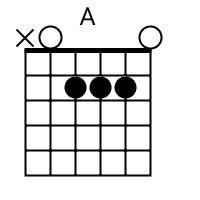
\includegraphics[width=3cm]{../Akordy/a.png}
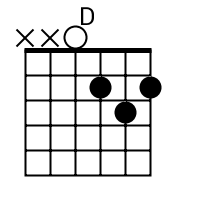
\includegraphics[width=3cm]{../Akordy/d.png}
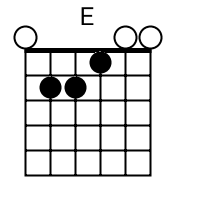
\includegraphics[width=3cm]{../Akordy/e.png}
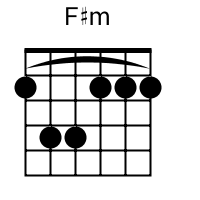
\includegraphics[width=3cm]{../Akordy/fxm.png}
\end{figure}
\newpage
\addcontentsline{toc}{section}{Náměšť}%%%%%%%%%%%%%%%%%%%%%%%%%%%%%%%%%%%%%%%%%%%%%%%%%%%%%
%			ŠABLONA PÍSNIČEK v. 18.09               %
%%%%%%%%%%%%%%%%%%%%%%%%%%%%%%%%%%%%%%%%%%%%%%%%%%%%%
% Tento soubor slouží jako (naučná) šablona, pomocí 
% které lze vytvářet zdrojové soubory k jednotlivým 
% písním.
%%%%%%%%%%%%%%%%%%%%%%%%%%%%%%%%%%%%%%%%%%%%%%%%%%%%%
%			Jak psát soubory songů?                 %
%%%%%%%%%%%%%%%%%%%%%%%%%%%%%%%%%%%%%%%%%%%%%%%%%%%%%
%	1. Text písně se začíná psát na místě START 
%	   a končí na místě END. Zbylý text ignorujte.
%	2. Jak bude vypadat pdf písně zjistíte po tom, 
%	   co soubor zkompilujete pomocí souboru   
%      ../Generator/generator. 
%	3. Při psaní dodržujte následující TeX pravidla:
%	 a) Nový řádek napíšete pomocí dvou odsazení 
%	    tedy dvou enterů.
%	 b) Nová sloka se píší pomocí \sloka a odsazení.
%		Refrén se píše jako \refren, v případě více 
%		refrénů \refren[č. refrénu].
%	 c) Akordy se píšou tak, že napíšete před slovo,
%	    kde chcete mít akord (bez mezery):
%		^{AKORD1\,AKORD2...}.
%	4. Pokud chcete ušetřit tvůrcům práci, tak 
%	   si přečtěte další poučný soubor o typografii 
%	   ../../Typo_pravidla.txt.
%	5. Akordy stačí psát jen do první sloky, když 
%	   se nezmění -- kytaristé to zvládnou
%	7. Název písně pište na místo [NÁZEV] a autora 
%	   pište na místo [AUTOR] 
%	7. Jak psát věci na české klávesnici:
%	   \ = alt gr + q; [/] = alt gr f/g; 
%      {/} = alt gr + b/n; ^ = alt gr + 3 , cokoliv
%%%%%%%%%%%%%%%%%%%%%%%%%%%%%%%%%%%%%%%%%%%%%%%%%%%%%
%			Jak kompilovat jednotlivé písně?        %
%%%%%%%%%%%%%%%%%%%%%%%%%%%%%%%%%%%%%%%%%%%%%%%%%%%%%
%	1. Více návodu je k tomuto napsáno v souboru 
%      ../Generator/generator. 
%%%%%%%%%%%%%%%%%%%%%%%%%%%%%%%%%%%%%%%%%%%%%%%%%%%%%
%			Jak kompilovat celý zpěvník?			%
%%%%%%%%%%%%%%%%%%%%%%%%%%%%%%%%%%%%%%%%%%%%%%%%%%%%%
%	1. Více návodu je k tomuto napsáno v souboru
%	   ../Cely_zpevnik/zpevnik.tex.
%%%%%%%%%%%%%%%%%%%%%%%%%%%%%%%%%%%%%%%%%%%%%%%%%%%%%
\begin{song}{title=\predtitle \centering Náměšť \\\large Jaroslav Hutka }  %% sem se napíše jméno songu a autor

\vspace*{.5cm}

\begin{centerjustified}
\nejnejvetsi
\sloka
/: ^{C}Krásný je ^*{\z Ami}vzduch , ^{Dmi}krásnější je ^{G}moře, :/

/: ^{C}co je ^*{\z A7}nejkrásnějš í, ^{F}co je ^*{\z G}nejkrásně jší --

-- ^{C \phantom{D} G\phantom{G}}usměvavé ^{C}tváře. :/

\sloka
/: Pevný je stůl, pevnější je hora, :/

/: co je nejpevnější, co je nejpevnější --

-- ta člověčí víra. :/

\sloka
/: Pustá je poušť i nebeské dálky, :/

/: co je nejpustější, co je nejpustější --

-- žít život bez lásky. :/

\sloka
/: Mocná je zbraň, mocnější je právo, :/

/: co je nejmocnější, co je nejmocnější --

-- pravdomluvné slovo. :/

\sloka
/: Velká je Zem, šplouchá na ní voda, :/

/: co je však největší, co je však největší --

-- ta lidská svoboda. :/

\end{centerjustified}
\setcounter{Slokočet}{0}
\end{song}
\newpage
\addcontentsline{toc}{section}{Nejlíp jim bylo}\begin{song}{title=\centering Nejlíp jim bylo \\\normalsize Mňága \& Žďorp  \vspace*{-0.3cm}}  %% sem se napíše jméno songu a autor
\moveright 5.5cm \vbox{      %Varianta č. 1  ---> Jeden sloupec zarovnaný na střed	

\sloka 
	Nejlíp jim ^{C\,Fmaj7}bylo,
	
	^{C}když ^{Fmaj7}nevěděli, co ^{C\,Fmaj7}dělaj, ^{C\,Fmaj7}
	
	jenom se ^{G}potkali 

	^{F}a neznělo to ^{C\,Fmaj}špatně. 

\sloka
	Tak se snažili 
	
	a opravdu si užívali,
	
	jenom existovali 
	
	a čas běžel skvěle.

\refren
	^{F}Nechám si projít ^{C}hlavou,
	
	^{G}kam všechny věci ^{Ami}plavou,
	
	^{F}jestli je všechno jen ^{C}dech

	^{G}tak jako kdysi v noci 

	^{Ami}spolu potmě na schodech. ^{C\,Fmaj7}

\sloka
	Pak se ztratili 

	a chvílema se neviděli,

	jenom si telefonovali 

	a byli na tom bledě.

\sloka
	A když se vrátili,
	
	už dávno nehořeli,

	jenom dál usínali

	chvíli spolu -- chvíli vedle sebe.

\refren

\sloka
	Nechej si projít hlavou,
	
	kam všechny věci věci plavou,
	
	jestli je všechno jen dech
	
	tak jako kdysi v noci 

	spolu potmě na schodech.



}
\setcounter{Slokočet}{0}
\end{song}
\newpage % Nevim presne, jak hrat... %Je to fakt dobrá písnička, já bych ji tam dal -- Jindra % Uz jsem na to prisel
\addcontentsline{toc}{section}{Pažitka}\begin{song}{title=\predtitle\centering Pažitka \\\large Xavier Baumaxa  \vspace*{-0.3cm}}  %% sem se napíše jméno songu a autor
\begin{centerjustified}

\sloka
Krajina ^*{A}sv ádí k podzimním ^{C#mi{\color{white}\_}\:\,}výletům,

tripům do ^{F#mi}mládí a častým ^*{D}úl etům.

Barevný ^*{A}lis tí je rázem ^{C#mi{\color{white}\_}\:\:}pestřejší,

hlavu ^{\:\:\,F#mi\z}ti~čistí,~no~a ty jsi ^*{D}by střejší.


\refren
/: ^*{A}Pa šuješ zážitky,

^*{E}pa šuješ všechno co se ^{F#mi}dá,\:\:\:\:

\phantom{.}

sáčky suchý pažitky,

^{D{\color{white}\_}}tomu se říká dobrá nálada. :/



\sloka
Hladina tůní pomalu vychladá,

je konec vůním a léto uvadá.

Na stehna fenek, dopadl dlouhý stín,

skončil čas trenek, ale já zas něco vymyslím.


\refren


\sloka
Cenzura.


\refren

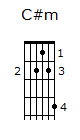
\includegraphics[width = 3cm]{../Akordy/cxm.png}
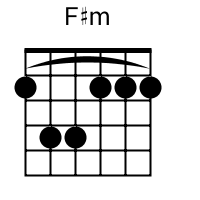
\includegraphics[width = 3cm]{../Akordy/fxm.png}


\end{centerjustified}
\setcounter{Slokočet}{0}
\end{song}
\newpage
\addcontentsline{toc}{section}{Perfect Day}\begin{song}{title=\centering Perfect Day \\\normalsize Lou Reed \vspace*{-0.3cm}}  %% sem se napíše jméno songu a autor
\moveright 2cm \vbox{      %Varianta č. 1  ---> Jeden sloupec zarovnaný na střed	
\begin{minipage}[t]{0.45\textwidth}\setlength{\parindent}{0.45cm}  %Varianta č. 2 --> Dva sloupce
\sloka 
	\textbf{E  Am  E  Am }

	^{Ami}Just a ^{D}perfect day, 

	^{G}Drink Sangria ^{C}in the park, 

	^{F}And then later, ^{Dmi}when it gets dark, 

	We go ^{E}home.
	 	
	^{Ami}Just a ^{D}perfect day, 

	^{G}Feed animals ^{C}in the zoo 

	^{F}Then later, ^{Dmi}a movie, too, 

	And then ^{E}home. 
 
 
\refren
	Oh ^{A}it's such a ^{D}perfect day, 

	I'm ^{C\# mi}glad I spent it with ^{D}you. ^{D\,\,D}

	^{A}Oh such a ^{E}perfect day, 

	You just ^{F\# mi}keep me ^{E}hanging ^{D}on, 

	You just ^{F\# mi}keep me ^{E}hanging ^{D}on. 
 
\sloka 
	Just a perfect day, 

	Problems all left alone, 

	Weekenders on our own. 

	It's such fun. 

	Just a perfect day, 

	You made me forget myself. 
	
	I thought I was someone else, 
	
	Someone good. 

\end{minipage}\begin{minipage}[t]{0.53\textwidth}\setlength{\parindent}{0.45cm}\vspace*{0.55cm}  % V případě varianty č.2 jde odsud text do pravé části

\refren 
	Oh it's such a perfect day, 
	
	I'm glad I spent it with you. 
	
	Oh such a perfect day, 
	
	You just keep me hanging on, 
	
	You just keep me hanging on. 
 

 
/: \textbf{F\# mi  E  D} :/

 
\sloka 
	/: ^{C\# mi}You're going to ^{G}reap 
	
	just what you ^{D}sow,  ^{D\,B\,A} :/
 
 	/: ^{C\# mi}You're going to ^{G}reap 
 	
 	just what you ^{D}sow,  ^{D\,B\,A} :/\\
 	
 	
\textbf{C\# mi   G   D   D   D   A }

\end{minipage}
}
\setcounter{Slokočet}{0}
\end{song}

\newpage
\addcontentsline{toc}{section}{Petěrburg}\begin{song}{title=\predtitle\centering Petěrburg  \\\large Jaromír Nohavica  \vspace*{-0.3cm}}  %% sem se napíše jméno songu a autor
\begin{centerjustified}
\nejnejvetsi

\sloka 
  ^{Ami}Když se snáší noc na střechy Petěrburgu, ^*{F}pa dá ^{E}na mě ^{Ami}žal,

  zatoulaný pes nevzal si ani kůrku ^*{F}ch leba, kterou ^*{E}js em mu ^{Ami}dal.

\refren
  /: ^*{C}Lá sku moji ^{Dmi\,\,\,}kníže ^{E}Igor si bere,
 
  ^{F{\color{white}\_}}nad sklenkou vodky ^{H7{\color{white}\_}}hraju ^{Adim\,\,}si ^{E}s revolverem,
  
  ^{Ami{\color{white}\_}}havran usedá na střechy Petěrburgu, ^{F{\color{white}\_}}čert ^{E}aby to ^{Ami}spral.

\sloka
  Nad obzorem letí ptáci slepí v záři červánků,
  
  moje duše, široširá stepi, máš na kahánku.

\refren
  /: Mému žalu na světě není rovno,
  
  vy jste tím vinna, Naděždo Ivanovno,
  
  vy jste tím vinna, až mě zítra najdou s dírou ve spánku. :/

\end{centerjustified}
\setcounter{Slokočet}{0}
\end{song}
\newpage
%POCITY -- od koho?
%POVĚSTE HO VEJŠ -- od koho?
\addcontentsline{toc}{section}{Rád vařim}%\documentclass[../main.tex]{subfiles}

\newcommand\tab[1][1cm]{\hspace*{#1}}
\begin{song}{title=\centering Rád vařim \\\normalsize MIDI LIDI \vspace*{-0.3cm}}  %% sem se napíše jméno songu a autor
\moveright 1cm \vbox{      %Varianta č. 1  ---> Jeden sloupec zarovnaný na střed	
\begin{minipage}[t]{0.48\textwidth}\setlength{\parindent}{0.45cm}  %Varianta č. 2 --> Dva sloupce

\sloka
^{Gmi}Rád ^{Cmi\,\,\,\,}vařim a ^{Gmi\,\,}vim, že to ^{Cmi\,\,\,\,}umim

a ^{Gmi\,\,\,\,\,\,\,\,}holkám ^{Cmi}se to ^{Dmi}líbí.

\phantom{.}

Rád vařím a vím, že to umím

a holkám se to líbí.

\phantom{.}

Rád vařím a vím, že to umím

a holkám se to líbí.

\phantom{.}

Rád vařím a vím, že to umím

a holkám se to líbí.

\phantom{.}

[Mezihra]

\sloka
Rád vařím a vím, že to umím

a holkám se to líbí.

\phantom{.}

Rád vařím a vím, že to umím

a holkám se to líbí.

\phantom{.}

Rád vařím a holkám vařím 

a holkám se to líbí.

\phantom{.}

Já rád vařím a holkám vařím 

a holkám se to líbí.


\sloka
Rád vařím a holkám vařím
 
a holkám se to líbí.

\phantom{.}

Rád vařím a holkám vařím 

a holkám se to líbí.

\phantom{.}

Já vařím a holkám vařím
 
a holkám se to líbí.

\phantom{.}

Rád vařím a holkám vařím 

a holkám se to líbí.

\phantom{.}

[Mezihra]

\end{minipage}\begin{minipage}[t]{0.48\textwidth}\setlength{\parindent}{0.45cm}\vspace*{0.55cm}  % V případě varianty č.2 jde odsud text do pravé části

\sloka
Rád vařím a vím, že to umím

a holkám se to líbí.

\phantom{.}

Rád vařím a holkám vařím 

a moc se mi to líbí.

\phantom{.}

Rád mlčím a doma trčím 

ale v práci mi to myslí.

\phantom{.}

Rád mlčím a doma trčím 

ale v práci mi to myslí.

\phantom{.}

Rány hojím, a proto za to stojím

a Vám všem se to líbí.

\phantom{.}

Rány hojím, a proto za to stojím 

a Vám všem se to líbí.

\end{minipage}
}
\setcounter{Slokočet}{0}
\end{song}
\newpage % Tezko se hraje
\addcontentsline{toc}{section}{Ráda se miluje}%\documentclass[../main.tex]{subfiles}

\begin{song}{title=\centering Ráda se miluje \\\normalsize Karel Plíhal  \vspace*{-0.3cm}}  %% sem se napíše jméno songu a autor
\moveright 4cm \vbox{      %Varianta č. 1  ---> Jeden sloupec zarovnaný na střed	

\refren
^{Hmi}Ráda se miluje, ^{A{\color{white}\_}}ráda ^{D}jí,

^{G{\color{white}\_}}ráda si ^{F#mi\,}jenom tak ^{Hmi{\color{white}\_}}zpívá, 

vrabci se na plotě ^{A\,{\color{white}\_}D\,}hádají, 

^{G{\color{white}\_\_}}kolik že ^{F#mi}času jí ^{Hmi{\color{white}\_}}zbývá.

\sloka
^{G}Než vítr dostrká k ^{D\,{\color{white}\_}}útesu ^{G}tu její legrační ^{{\color{white}\_}D\,\,F#mi}bárku 

a ^{Hmi\,\,}Pámbu si ve svým ^{A{\color{white}\_}D}notesu ^{G{\color{white}\_\_}}udělá ^{F#mi}jen další ^{Hmi\,\,}čárku.

\refren

\sloka
Psáno je v nebeské režii, a to hned na první stránce, 

že naše duše nás přežijí v jinačí tělesný schránce. 

\refren

\sloka
Úplně na konci paseky, tam, kde se ozvěna tříští, 

sedí šnek ve snacku pro šneky -- snad její podoba příští. 


\refren

}
\setcounter{Slokočet}{0}
\end{song}

\newpage
%SEDMIKRÁSKA -- od koho?
\addcontentsline{toc}{section}{Severní Vítr}%%%%%%%%%%%%%%%%%%%%%%%%%%%%%%%%%%%%%%%%%%%%%%%%%%%%%
%			ŠABLONA PÍSNIČEK v. 18.09               %
%%%%%%%%%%%%%%%%%%%%%%%%%%%%%%%%%%%%%%%%%%%%%%%%%%%%%
% Tento soubor slouží jako (naučná) šablona, pomocí 
% které lze vytvářet zdrojové soubory k jednotlivým 
% písním.
%%%%%%%%%%%%%%%%%%%%%%%%%%%%%%%%%%%%%%%%%%%%%%%%%%%%%
%			Jak psát soubory songů?                 %
%%%%%%%%%%%%%%%%%%%%%%%%%%%%%%%%%%%%%%%%%%%%%%%%%%%%%
%	1. Text písně se začíná psát na místě START 
%	   a končí na místě END. Zbylý text ignorujte.
%	2. Jak bude vypadat pdf písně zjistíte po tom, 
%	   co soubor zkompilujete pomocí souboru   
%      ../Generator/generator. 
%	3. Při psaní dodržujte následující TeX pravidla:
%	 a) Nový řádek napíšete pomocí dvou odsazení 
%	    tedy dvou enterů.
%	 b) Nová sloka se píší pomocí \sloka a odsazení.
%		Refrén se píše jako \refren, v případě více 
%		refrénů \refren[č. refrénu].
%	 c) Akordy se píšou tak, že napíšete před slovo,
%	    kde chcete mít akord (bez mezery):
%		^{AKORD1\,AKORD2...}.
%	4. Pokud chcete ušetřit tvůrcům práci, tak 
%	   si přečtěte další poučný soubor o typografii 
%	   ../../Typo_pravidla.txt.
%	5. Akordy stačí psát jen do první sloky, když 
%	   se nezmění -- kytaristé to zvládnou
%	7. Název písně pište na místo [NÁZEV] a autora 
%	   pište na místo [AUTOR] 
%	7. Jak psát věci na české klávesnici:
%	   \ = alt gr + q; [/] = alt gr f/g; 
%      {/} = alt gr + b/n; ^ = alt gr + 3 , cokoliv
%%%%%%%%%%%%%%%%%%%%%%%%%%%%%%%%%%%%%%%%%%%%%%%%%%%%%
%			Jak kompilovat jednotlivé písně?        %
%%%%%%%%%%%%%%%%%%%%%%%%%%%%%%%%%%%%%%%%%%%%%%%%%%%%%
%	1. Více návodu je k tomuto napsáno v souboru 
%      ../Generator/generator. 
%%%%%%%%%%%%%%%%%%%%%%%%%%%%%%%%%%%%%%%%%%%%%%%%%%%%%
%			Jak kompilovat celý zpěvník?			%
%%%%%%%%%%%%%%%%%%%%%%%%%%%%%%%%%%%%%%%%%%%%%%%%%%%%%
%	1. Více návodu je k tomuto napsáno v souboru
%	   ../Cely_zpevnik/zpevnik.tex.
%%%%%%%%%%%%%%%%%%%%%%%%%%%%%%%%%%%%%%%%%%%%%%%%%%%%%
\begin{song}{title=\predtitle \centering Severní vítr \\\large Zdeněk Svěrák \& Jaroslav Uhlíř }  %% sem se napíše jméno songu a autor

\vspace*{.5cm}

\begin{centerjustified}
\vetsi
\sloka
Jdu ^{C\z}s~děravou patou, mám ^{Ami\z }horečku zlatou,

jsem ^{F\z}chudý, jsem sláb, ^*{\z C}nemoc en.

Hlava mě pálí a ^{Ami\z}v~modravé dáli se ^{F\z}leskne

a ^{G7\z}třpytí můj ^{C\z}sen.

\sloka
Kraj pod sněhem mlčí, tam stopy jsou vlčí,

tam zbytečně budeš mi psát,

sám v dřevěné boudě sen o zlaté hroudě

já nechám si tisíckrát zdát.

\refren
^{C\z}Severní ^{C7\z}vítr je ^{F}krutý,

^{C\z}počítej, lásko má, ^{G7\z}s~tím,

^{C\z}k~nohám Ti ^{C7\z}dám zlaté ^{F\z}pruty

nebo se ^{C\z}vůbec ^{G7 \, C\z}nevrátím.

\sloka
Tak zarůstám vousem a vlci už jdou sem,

už slyším je výt blíž a blíž.

Už mají mou stopu, už větří, že kopu

svůj hrob a že stloukám si kříž.

\sloka
Zde leží ten blázen, chtěl dům a chtěl bazén

a opustil tvou krásnou tvář.

Má plechovej hrnek a pár zlatejch zrnek

a nad hrobem polární zář.

\refren

\end{centerjustified}
\setcounter{Slokočet}{0}
\end{song}
\newpage
\addcontentsline{toc}{section}{Sound Of Silence}%\documentclass[../main.tex]{subfiles}

\begin{song}{title=\centering Sound Of Silence \\\normalsize Simon \& Garfunkel  \vspace*{-0.3cm}}  %% sem se napíše jméno songu a autor
\moveright \stred \vbox{      %Varianta č. 1  ---> Jeden sloupec zarovnaný na střed	
\sloka
   ^{Ami}Hello darkness my ^{G}old friend
   
   I've come to talk with you ^{Ami}again
   
   because a ^{C}vision softly ^{F C}creeping
   
   left it seeds while I was ^{F C}sleeping.
   
   And the ^{F}vision that was planted in my ^{C}brain 
   
   still ^{Ami}remains ^{C}within the ^{G}sound of ^{Ami}silence.

\sloka
   In restless dreams I walked alone, 
   
   narrow streets of cobble-stone ,
   
   'neath the halo of a street lamp 
   
   I turned my collar to the cold and damp.
   
   When my eyes were stabbed by the flash of a neon light 
   
   that spilt the night and touched the sound of silence.
   
\sloka
   And in the naked light I saw 
   
   ten thousand people maybe more 
   
   People talking without speaking,
   
   people hearing without listening,
   
   people writing songs that voices never share,
   
   and no one dare disturb the sound of silence.
   
\sloka
   \uv{Fools!} said I \uv{you do not know
   
   silence like a cancer grows 
   
   hear my words that I might teach you 
   
   take my arms that I might reach you.} 
   
   But my words like silent raindrops fell 
   
   and echoed in the wells of silence. 
   
\sloka
   And the people bowed and prayed 
   
   to the neon god they made 
   
   and the sign flashed out its warning 
   
   in the words that it was forming and the sign said: 
   
   \uv{The words of the prophets are written on the subway walls 
   
   and tenament halls} and whisper'd in the sound of silence. 
   

}
\setcounter{Slokočet}{0}
\end{song}
\newpage
\addcontentsline{toc}{section}{Stánky}\begin{song}{title=\predtitle\centering Stánky \\\large Nedvědi \vspace*{-0.3cm}}  %% sem se napíše jméno songu a autor
\begin{centerjustified}
\nejnejvetsi

\sloka
	^*{D}U\: stánků ^{G}na levnou krásu

	^{D\z}postávaj a ^{Gmi\z}smějou se času,

	s ^{D\z}cigaretou a s ^{A7\z}holkou, co nemá kam ^{D}jít.

\sloka
	Skleniček pár a pár tahů z trávy,
   	
   	uteče den jak večerní zprávy,
   	
   	neuměj' žít a bouřej' se a neposlouchaj'.

\refren
	^{G}Jen zahlídli svět, maj' ^{A}na duši vrásky,

	tak ^{D\z}málo je, ^{Gmi}málo je lásky,

	^{D\z}ztracená víra ^{A7\z}hrozny z vinic ^{{\color{white}\_\_\_}D}neposbírá.

\sloka
	U stánků na levnou krásu
   	
   	postávaj' a ze slov a hlasů
   	
   	poznávám, jak málo jsme jim stačili dát.

\refren

\refren


\end{centerjustified}
\setcounter{Slokočet}{0}
\end{song}
\newpage
%STROM
\addcontentsline{toc}{section}{Studený nohy}\begin{song}{title=\predtitle\centering Studený nohy \\\large Radůza\vspace*{-0.3cm}}  %% sem se napíše jméno songu a autor
\begin{centerjustified}
\nejvetsi

\predehra 
/: \textbf{A\,D\,E\,H\,A\,D\,E} :/

\sloka
	^{Ami} ^ {Emi}Prší, ^{Dmi\z}choulím se ^{Emi\z}do~svrchníku,

	^{Ami\z}než~se ^{Emi\z}otočím ^{F}na ^{G}podpatku
	
	zalesknou se světla na chodníku,
   	
   	jak pětka na věčnou oplátku.

\sloka
	Slyším kroky zakletejch panen,
   	
   	to je vínem, to je ten pozdní sběr,
   
   	každá kosa najde svůj kámen,
   	
   	to je vínem, ber mě, ber.

\refren
	Studený ^{F\z}nohy ^{E\z}schovám doma ^{Ami\z}pod~peřinou

	a ráno ^{F\z}kafe dám si ^{E\z}hustý jako ^{Ami\z}tér,\:\:\:\:

	přežiju ^{F\z}tuhle ^{\z E}neděli tak jako ^{Ami\z}každou jinou,

	na koho ^{F\z}slovo padne, ^{E}ten je ^*{\z D}solitér . ^{Ami} 

\sloka
	Broukám si píseň o klokočí,
   	
   	prší a dlažba leskne se,
   	
   	je chladno a hlava, ta se točí,
   	
   	jak světla na plese.

\refren

\sloka
	Tak mám a nebo nemám kliku,
   
   	zakletá panna směje se
   	
   	a moje oči, lesknou se na chodníku,
   	
   	jak světla na plese.

\refren

\end{centerjustified}
\setcounter{Slokočet}{0}
\end{song}
\newpage
\addcontentsline{toc}{section}{To ta He\v lpa}\begin{song}{title=\predtitle\centering To ta He\v lpa \\\large  \vspace*{-0.3cm}}  %% sem se napíše jméno songu a autor
\begin{centerjustified}
\nejnejvetsi

\sloka 
	^{Dmi}To ta ^{G\z}Helpa, ^{Dmi}to ta ^{G\z}Helpa, ^{Dmi\,}to je ^{A7\z}pekné ^{Dmi\,\,}mesto.

	^{Dmi}A v tej ^{G\z}Helpe, ^{Dmi}a v tej ^{G\z}Helpe ^{Dmi\,\z}švarných ^{A7\z}chlapcov ^{Dmi}je sto.

	/: ^{B\z}Koho ^{C7}je sto, ^{F\z}toho je sto, ^{C}nie po mojej ^{\,\,\,F\,\,A7}vóli,

	^{Dmi}len za ^{G\z}jednym, ^{Dmi}len za ^{G\z}jednym ^{Dmi\,A7{\color{white}\_\_}}srdiečko ma ^{Dmi\z}boli.~:/


\sloka
	Za Janíčkom, za Palíčkom krok by něspravila,
	
	za Ďuríčkom, za Mišíčkom Dunaj preskočila.

	/: Dunaj, Dunaj, Dunaj, Dunaj, aj to širé pole,
	
	len za jedním, len za jedním, počešenie moje. :/

\end{centerjustified}
\setcounter{Slokočet}{0}
\end{song}
\newpage
%TOHLETO BY JEŽÍŠ NEŘEŠIL
\addcontentsline{toc}{section}{Trezor}\begin{song}{title=\centering Trezor \\\normalsize Karel Gott  \vspace*{-0.3cm}}  %% sem se napíše jméno songu a autor
\moveright 3cm \vbox{      %Varianta č. 1  ---> Jeden sloupec zarovnaný na střed	

\sloka 
	^{D}Ze zdi na mě tupě zírá ^{G}po trezoru temná díra,

	^{E7{\color{white}\_\_\_}}poznám tedy bez nesnází, ^{A7}že tam nepochybně něco schází.

	^{D}Ve zdi byl totiž po dědovi ^{G{\color{white}\_}}velký trezor ocelový.

	^{A7{\color{white}\_}}Mám tedy ztrátu zdánlivě ^{{\color{white}\_\_\_}D}minimální.
      
\sloka
	^{D}Na to že ^{A7{\color{white}\_\_\_}}náhodně v krámě vášnivé dámě ^{D{\color{white}\_}}padl jsem za ^{Hmi}trofej,

	^{E7{\color{white}\_\_}}tvrdila pevně: ,,Přijdu tě levně, ^{A7{\color{white}\_\_\_}}nezoufej!`` Ó jé, jé, jé, jé.

	^{D{\color{white}\_\_}}Jenže potom v naší vile ^{G{\color{white}\_\_\_}}chovala se zhůvěřile,

	^{E7}aby měla správné klima, ^{A7}dal jsem ji do trezoru, ať v klidu dřímá.
      
\refren
	^{D{\color{white}\_\_\_}}Spánku se bráním už noc pátou, ^{G}ne ale žalem nad tou ztrátou,

	^{A7}jen hynu bázní, že kasař úlovek ^{G D}vrátí.
      
\sloka = 2.
      
\refren


}
\setcounter{Slokočet}{0}
\end{song}

\newpage
\addcontentsline{toc}{section}{Už to nenapravím}\begin{song}{title=\predtitle\centering Už to nenapravím \\\large Jaroslav Samson Lenk  \vspace*{-0.3cm}}  %% sem se napíše jméno songu a autor
\begin{centerjustified}

\refren /: ^{Ami\z}Vap~tada dap\elipsa\dots ^{D\,\,F\,\,E} :/

\sloka
	V ^{Ami}devět hodin dvacet pět mě ^{D\z}opustilo štěstí, 
	
	ten ^{F\z}vlak, co jsem jím měl jet, na koleji ^{E\z}dávno ^{E7\z}nestál.
	
	V ^{Ami}devět hodin dvacet pět ^{D\z}jako bych dostal pěstí,
	
	já ^{F}za hodinu na náměstí měl jsem ^{E\z}stát, ale ^{E7\z}v~jiným městě.
	
	
	Tvá ^{Ami}zpráva zněla prostě a byla tak krátká,
		
	že ^{Dmi\z}stavíš se jen na skok, že nechalas mi vrátka ^{G\z}zadní otevřená, ^{E\z}zadní otevře^{E7}ná.
	
	Já ^{Ami\z}naposled tě viděl když ti bylo dvacet 
	
	a ^{Dmi\z}to~si tenkrát řekla, že už se nechceš vracet, ^{G}že si unavená, ^{E}ze mě unave^{E7}ná.
	


\refren

\sloka
	Já čekala jsem, hlavu jako střep a zdálo se, že dlouho, 
	
	snad může za to vinný sklep, že člověk často sleví.
	
	Já čekala jsem, hlavu jako střep, podvědomou touhou, 
	
	já čekala jsem dobu dlouhou víc než dost, kolik přesně nevím.


	Pak jedenáctá bila a už to bylo passé, 

	já dřív jsem měla vědět, že vidět tě chci zase, že láska nerezaví, láska nerezaví.
	
	Ten dopis, co jsem psala byl dozajista hloupý,
	
	byl odměřený moc, na vlídný slovo skoupý, už to nenapravím, už to nenapravím.
	


\refren


\end{centerjustified}
\setcounter{Slokočet}{0}
\end{song}
\newpage
\addcontentsline{toc}{section}{Velmi nesmělá}\begin{song}{title=\predtitle\centering Velmi nesmělá \\\large Jablkoň  \vspace*{-0.3cm}}  %% sem se napíše jméno songu a autor
\begin{centerjustified}

\begin{varwidth}[t]{0.48\textwidth}\setlength{\parindent}{0.45cm}  %Varianta č. 2 --> Dva sloupce
\sloka
	^{Ami\z}Potkali se v pondělí, v ^{Emi Ami\z}pondělí.\:\:\:
	
	^{Ami}Byli velmi nesmělí, ^{G\,\,\,\,\,\,\,\,E7}nesmělí,
	
	^{C}a tak oba dělali, ^{Dmi7\,Esmi7\,Emi7}dělali
	
	^{Ami\,\,}jakoby se neznali, ^{Emi Ami\z}neznali.\:\:\:
	
	
\sloka
	V úterý sebral odvahu, odvahu.
	
	Odhodlal se k pozdravu, pozdravu.
	
	A pak v citové panice, panice
	
	prchali oba k mamince, mamince.

\refren
	^{C{\color{white}\_\_}E\,\,}Semafor popásá ^{F\,\,\,\,\,\,\,}chodce,
	
	motorky ^{C\,\,\,\,}auta ^{G\,\,\,\,\,\,\,\,\,C\,\,}tramvaje.
	
	A všechny ^{E\,\,\,\,\,\,}cesty dneska ^{F\,\,\,\,\,\,\,}vedou
	
	/: ^{C}do pekla i ^{G}do ^{C Ami\z}ráje.~:/
	
\sloka
	Ve středu spolu postáli, postáli,
	
	dívali se do dáli, do dáli.
	
	A do dáli se dívali, dívali
	
	i když už spolu nestáli, nestáli.
	

\sloka
	Ve čtvrtek přišel první zvrat,
	
	první zvrat,
	
	prohlásil že má ji rád, má ji rád.
	
	A ona špitla do ticha, do ticha,
	
	že na ni moc pospíchá, pospíchá

\refren

\sloka
	V pátek to vzal útokem, útokem,
	
	jak tak šli krok za krokem, za krokem.
	
	Přesně v šestnáct dvacet pět,

	dvacet pět
	
	zavadil loktem o loket, o loket.

\end{varwidth}\mezisloupci\begin{varwidth}[t]{0.48\textwidth}\setlength{\parindent}{0.45cm}\vspace*{0.55cm}  % V případě varianty č.2 jde odsud text do pravé části
\vspace*{-.185cm}
\sloka
	V sobotu ji chyt za ruku, za ruku.
	
	Hlavou jí kmitlo je to tu, je to tu.
	
	A jak hodiny běžely, běžely,
	
	drželi se drželi, drželi.


\refren
	
\sloka
	V neděli už věděli, věděli,

	že jsou možná dospělí, dospělí.
	
	A tak při sedmém pokusu, pokusu,
	
	dal jí pusu na pusu, na pusu.


\sloka
	Když zas přišlo pondělí, pondělí,
	
	příšerně se styděli, styděli.
	
	A tak oba dělali, dělali,
	
	jakoby se neznali, neznali.

\phantom{.}

\phantom{.}

 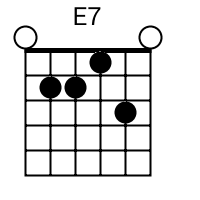
\includegraphics[width = 3cm]{../Akordy/e7.png}
 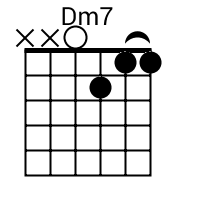
\includegraphics[width = 3cm]{../Akordy/dm7.png}

 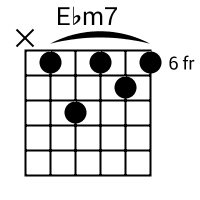
\includegraphics[width = 3cm]{../Akordy/esm7.png}
 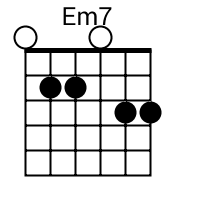
\includegraphics[width = 3cm]{../Akordy/em7.png}



\end{varwidth}

\end{centerjustified}
\setcounter{Slokočet}{0}
\end{song}
\newpage
\addcontentsline{toc}{section}{What Shall We Do With the Drunken Sailor}\begin{song}{title=\predtitle\centering What Shall We Do With the Drunken Sailor \\\large   \vspace*{-0.3cm}}  %% sem se napíše jméno songu a autor
\begin{centerjustified}

\sloka
	^{Dmi}What shall we do with a drunken sailor,

	^{C\z }What shall we do with a drunken sailor,

	^{Dmi}What shall we do with a drunken sailor,

	^{F\z }early ^{A7}in the ^{Dmi\z }morning?


\refren
	^{Dmi\z }Hooray and up she rises, ^{C\z }hooray and up she rises.

	^{Dmi\z }Hooray and up she rises ^{F\z }early ^{A7}in the ^{Dmi\z }morning.


\sloka
	/: Put him in the longboat till he's sober, :/

	Put him in the longboat till he's sober

	Early in the morning.


\refren

\sloka
	/: Pull out the plug and wet him all over, :/
	
	Pull out the plug and wet him all over
	
	Early in the morning.

\refren

\sloka
	/: Put him in the scuppers with hose-pipe on him, :/
	
	Put him in the scuppers with hose-pipe on him
	
	Early in the morning.

\refren

\sloka
	/: Heave him by the leg in running bowline, :/

	Heave him by the leg in running bowline

	Early in the morning.

\refren

\sloka
	/: Tie him to the taffrail when she's yardarm under, :/

	Tie him to the taffrail when she's yardarm under

	Early in the morning.

\refren

\end{centerjustified}
\setcounter{Slokočet}{0}
\end{song}
\newpage
\addcontentsline{toc}{section}{Zatanči}\begin{song}{title=\centering Zatanči \\\normalsize Jaromír Nohavica  \vspace*{-0.3cm}}  %% sem se napíše jméno songu a autor
\moveright \stred \vbox{      %Varianta č. 1  ---> Jeden sloupec zarovnaný na střed	

\sloka
^{Emi G}Zatanči, má milá, ^{D{\color{white}\_\_}}zatanči ^{Emi}pro mé oči,

^{{\color{white}\_\_}G}zatanči a vetkni nůž ^{D}do mých ^{Emi}zad.

Ať tvůj ^{G}šat, má milá, ať ^{D}tvůj šat ^{Emi}na zemi skončí,

ať tvůj ^{G}šat, má milá, ^{D}rázem je ^{Emi}sňat.

\refren
^{Emi G}Zatanči, jako se ^{D{\color{white}\_}}okolo ^{Emi\,\,}ohně tančí,

^{{\color{white}\_\_}G}zatanči jako ^{D{\color{white}\_\_}}na\,\,vodě ^{Emi}loď,

^{{\color{white}\_\_}G}zatanči jako to ^{D}slunce ^{Emi}mezi pomeranči,

^{{\color{white}\_\_}G}zatanči, a ^{D}pak ke mně ^{Emi}pojď.

\phantom{.}

\textbf{Mezihra}

\sloka
Polož dlaň, má milá, polož dlaň na má prsa,

polož dlaň nestoudně na moji hruď.

Obejmi, má milá, obejmi moje bedra,

obejmi je pevně a mojí buď.

\refren

\phantom{.}

\textbf{Mezihra}

\sloka
Nový den než začne, má milá, nežli začne,

nový den než začne, nasyť můj hlad.

Zatanči, má milá, pro moje oči lačné,

zatanči a já budu ti hrát.

\refren

\refren
}
\setcounter{Slokočet}{0}
\end{song}
\newpage
%ŽELVA




%\begin{song}{title=\centering Strum patterns \\\normalsize Jak hrát na kytaru pravou rukou \vspace*{-0.3cm}}  %% sem se napíše jméno songu a autor

\newcommand{\up}{$\uparrow$} %Brnknutí dolů
\newcommand{\dn}{$\downarrow$} %Brnknutí nahoru
\newcommand{\x}{$\times$} %Ztlumení strun 
\newcommand{\tu}{\textunderscore} % Nehraní ničeho
\centering
\mezera 

%\setlength{\arrayrulewidth}{.1em}
\renewcommand{\arraystretch}{1.4}
\begin{tabular}{l  l  l}
\hline\hline 
Č. & Jak hrát & Kde se vyskytuje  \\ \hline
1  & \dn \up \dn \up \dn \up & základní styl brnkání, který lze zahrát téměř v~každé situaci\\
2  & \dn \tu \dn \up \dn \tu \dn \tu \dn & např. v~písni Slavíci z Madridu  \\
3  & \dn \tu \tu \tu \dn \tu \dn & např. v~písni Knockin' On Heaven's Door  \\
4  & \dn \x  \up \dn \up \dn & např. v~písni Dezolát \\
5  & \dn \up \dn \tu \dn \up & např. v~písni Cesta do Jenkovic \\
6  & \dn \tu \dn \up \tu \up \dn \up & lze hrát např. v~refrénu Cesty do Jenkovic \\
7  & \dn \tu \dn \tu \dn \up \dn \up & lze hrát např. v~refrénu Cesty do Jenkovic \\
\hline \hline
\end{tabular}



	
\setcounter{Slokočet}{0}
\end{song}


\newpage

\pagestyle{empty}

% Aby byla titulni strana a strana s akordy na coveru

\phantom{.}
\newpage

\phantom{.}
\newpage

%%%%%%%%%%%%% Přehled akordů %%%%%%%%%%%%%%%%
\newgeometry{top=0cm, bottom = 0cm, left = 0cm, right = 0cm}
\thispagestyle{empty}
\begin{figure}[h]
\centering
% PŘEHLED
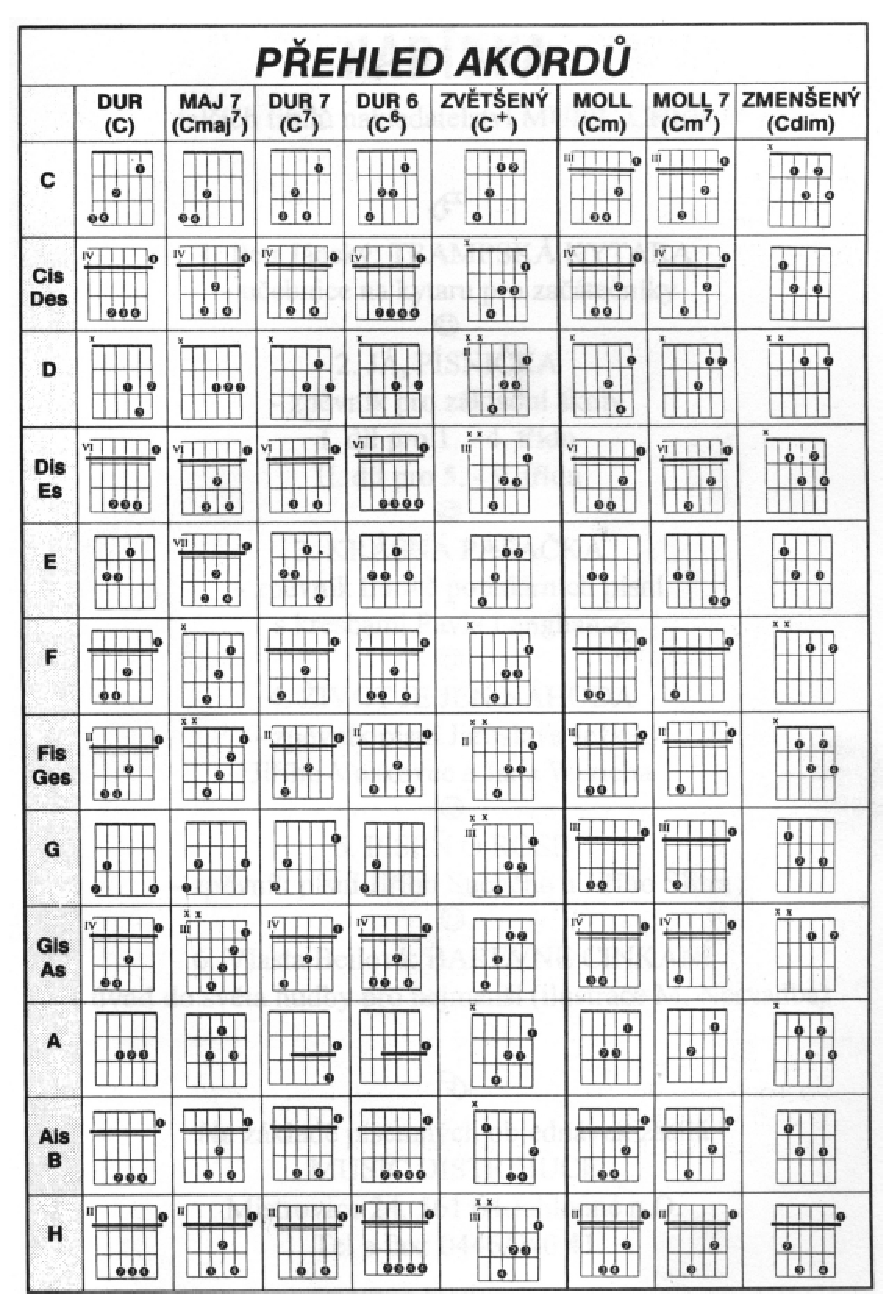
\includegraphics[height=\textheight]{../Akordy/AAAkordy3.pdf}
\end{figure}



\end{document}

